\documentclass{article}

% if you need to pass options to natbib, use, e.g.:
%     \PassOptionsToPackage{numbers, compress}{natbib}
% before loading neurips_2019

% ready for submission
% \usepackage{neurips_2019}

% to compile a preprint version, e.g., for submission to arXiv, add add the
% [preprint] option:
%     \usepackage[preprint]{neurips_2019}

% to compile a camera-ready version, add the [final] option, e.g.:
     \usepackage[final]{neurips_2019}

% to avoid loading the natbib package, add option nonatbib:
%     \usepackage[nonatbib]{neurips_2019}

\usepackage[utf8]{inputenc} % allow utf-8 input
\usepackage[T1]{fontenc}    % use 8-bit T1 fonts
\usepackage{hyperref}       % hyperlinks
\usepackage{url}            % simple URL typesetting
\usepackage{booktabs}       % professional-quality tables
\usepackage{amsmath,amsfonts,amssymb,amsthm}       % blackboard math symbols
\usepackage{nicefrac}       % compact symbols for 1/2, etc.
\usepackage{microtype}      % microtypography
\usepackage{multirow}
\usepackage{bbm}
\usepackage{graphicx}

\title{Graph Embedding with Personalized Context Distribution}


% The \author macro works with any number of authors. There are two commands
% used to separate the names and addresses of multiple authors: \And and \AND.
%
% Using \And between authors leaves it to LaTeX to determine where to break the
% lines. Using \AND forces a line break at that point. So, if LaTeX puts 3 of 4
% authors names on the first line, and the last on the second line, try using
% \AND instead of \And before the third author name.

\author{
Di Huang, Yuzhong Huang, Kexuan Sun, Zihao He}

\begin{document}



\maketitle

\begin{abstract}
Graph representation learning is a task of embedding graph nodes in a low-dimensional latent space with vectors. 
%Especially random walk based approaches gained traction for its scalability for large-scale graphs while preserving high-order proximity. 
However, real networks vary in size and structural properties. Heavily relying on hyper-parameters, certain random walk based approaches are not easily applicable due to its long hyper-parameter searching process. In this work, we improve WatchYourStep and learn graph embedding via a node-personalized context attention learning process. We replace the sharing context distribution with learnable personalized context distribution for each individual node. We evaluate our model on seven real networks and show that our methods outperforms state-of-the-art WatchYourStep on both link prediction and node classification tasks. We further provide analysis on learnt node context distribution and its correlation with graph structural properties.
\end{abstract}

\section{Introduction}

Graph embedding aims to learn a vector representation for each node in the graph, while preserving its structure information. Such embedding can been used in various downstream applications, such as node classification, link prediction and graph. Existing works can be divided into three main categories: matrix factorization, randon walks and deep learning models. Random walks based methods such as DeepWalk~\cite{perozzi2014deepwalk} and Node2vec~\cite{grover2016node2vec} especially gained great attraction for its scalability for large-scale graphs while preserving high-order proximity.

However, since many random walk based approaches significantly depend on their hyper-parameters settings such as the length of walk $C$ which may vary on different graphs. To solve such bottleneck, WatchYourStep~\cite{abu2018watch} extends a fixed value of $C$ to a trainable attention-based context distribution $\mathbf{Q}$. Regardless of its efficiency on various tasks, it focuses on the difference between graphs but does not take the difference between nodes into consideration. Indeed, nodes from the same graph may have distinct characteristics and thus play distinct roles. For example, a small number of nodes can have much higher degree than any other nodes.

Instead of learning an attention-based context distribution for a graph, we therefore propose a graph embedding method that learns a context distribution for each individual node. We parameterize a context distribution into three different formats and compare them with other state-of-the-art graph embedding methods on both link prediction and node classification tasks. The experimental results indicate the superiority of our proposed method. Furthermore, we provide analysis on learnt node context distribution and its correlation with graph structural properties, which may also potentially open up a new research direction in other embedding learning relate domains such as natural language processing. 


% HZH

% Graph embedding aims to learn a vector representation of each node in graph, while preserving its structural information. Its usefulness has been demonstrated in various downstream applications such as node classification~\cite{} and link prediction~\cite{}.
% Recently, dramatic advancements in graph embedding have been made in many existing works, such as DeepWalk~\cite{} and node2vec~\cite{}. 
% % The usefulness of graph embeddings has been shown in various downstream applications, such as node classification and link prediction. Therefore, there have been dramatic advancements in learning graph embedding, such as DeepWalk~\cite{} and node2vec~\cite{}.


% However, since many random walk based approaches significantly depend on their hyper-parameters settings such as the length of walk $C$ which may vary on different graphs. To solve such bottleneck, WatchYourStep~\cite{abu2018watch} extends a fixed value of $C$ to a trainable attention-based context distribution $\mathbf{Q}$. Regardless of its efficiency on various tasks, it focuses on the difference between graphs but does not take the difference between nodes into consideration. Indeed, nodes from the same graph may have distinct characteristics and thus play distinct roles. For example, a small number of nodes can have much higher degree than any other nodes. Ignoring such heterogeneity is prone to cause a inferior performance.

%As a matter of fact, a vast majority of these methods that stem from random walk significantly depend on settings of their hyper-parameters, such as the length of walk $C$ that may vary among different graphs. As a result, the tuning of $C$ involves tremendous trial-and-error and is usually time-consuming.
%To solve such a bottleneck, WatchYourStep~\cite{abu2018watch} extends a pre-defined $C$ to a trainable attention-based context distribution parameterized by a learnable vector $\mathbf{Q}$, which aims to capture the subtle but non-trivial dissimilarity of nodes through an automatic manner. 

%In spite of its capacity of considering the dissimilarity of different graphs, WatchYourStep fails to take the difference between nodes into consideration. Indeed, nodes from the same graph may play different roles displaying distinct characteristics, including the length of walk $C$. For example, a small number of nodes can have much higher degree than other nodes in a graph. Ignoring such heterogeneity is prone to cause a inferior performance.

%Instead of learning an attention-based context distribution for a graph, we therefore propose a graph embedding method that learns a context distribution for each individual node. We parameterize a context distribution into three different formats and compare them with other state-of-the-art graph embedding methods on both link prediction and node classification tasks. The experimental results indicate the superiority of our proposed method. Furthermore, we provide analysis on learnt node context distribution and its correlation with graph structural properties, which may also potentially open up a new research direction in other embedding learning relate domains such as natural language processing. 


% HZH

% Graph embedding aims to learn a vector representation of each node in graph, while preserving its structural information. Its usefulness has been demonstrated in various downstream applications such as node classification~\cite{} and link prediction~\cite{}.
% Recently, dramatic advancements in graph embedding have been made in many existing works, such as DeepWalk~\cite{} and node2vec~\cite{}. 
% % The usefulness of graph embeddings has been shown in various downstream applications, such as node classification and link prediction. Therefore, there have been dramatic advancements in learning graph embedding, such as DeepWalk~\cite{} and node2vec~\cite{}.

% As a matter of fact, a vast majority of these methods that stem from random walk significantly depend on settings of their hyper-parameters, such as the length of walk $C$ that may vary among different graphs. As a result, the tuning of $C$ involves tremendous trial-and-error and is usually time-consuming.
% Fortunately, WatchYourStep~\cite{} extends a pre-defined $C$ to a trainable attention-based context distribution parametrized by a learnable vector $\mathbf{Q}$, which aims to capture the subtle but non-trivial heterogeneity hidden in topology through an automatic manner. Such a graph attention model manages to achieve significant error reduction in different tasks~\cite{}.

% In spite of its capacity of considering the dissimilarity of different graphs, WatchYourStep fails to take the difference between nodes into consideration. Indeed, nodes from the same graph may play different roles displaying distinct characteristics, including the length of walk $C$. For example, a small number of nodes can have much higher degree than other nodes in a graph. Ignoring such heterogeneity is prone to cause a inferior performance.
% % For example, some nodes with a higher degree may have a larger context to look at while other more disconnected nodes may have a smaller one. As a matter of fact, a global context distribution presumes the homogeneity over various nodes, which tend to not hold water. In contrast, our method endows each node with sufficient autonomy to explore their personalized optimal context distribution parametrized by only a few learnable parameters, the quantity of which is fairly tractable.

% To this end, in this paper, instead of learning an attention-based context distribution for the entire graph, we therefore propose a graph embedding method that learns a context distribution for each individual node. Specifically, we parametrize a context distribution into three different forms and compare them with other state-of-the-art graph embedding methods on both link prediction and node classification tasks. Extensive experimental results indicate the superiority of our proposed method on both link prediction and node classification, which may also potentially open up a new research direction in other domains involving embedding learning such as natural language processing. 
\section{Methodology}


\subsection{Objective Function}
Similar to WatchYourStep, we use negative log graph likelihood(NLGL) as our log function:

$\displaystyle\min_{\mathbf{L},\mathbf{R},\mathbf{Q}}\alpha(\|\mathbf{L}\|_2^2 + \|\mathbf{R}\|_2^2 ) + \beta\|\mathbf{Q}\|_2^2 +\|-\mathbb{E}[\mathbf{D};\mathbf{Q}]\circ\log(\sigma(\mathbf{L}\times\mathbf{R}^\intercal)) -\mathbbm{1}[\mathbf{A}=0]\circ\log(1-\sigma(\mathbf{L}\times\mathbf{R}^\intercal)) \|_1$
where $\mathbb{E}[\mathbf{D};\mathbf{Q}] = \tilde{\mathbf{P}}^{(0)}\displaystyle\sum_{k=1}^{C}p(Q)_k(\mathcal{T})^k$. A is graph adjacency matrix and $\tilde{\mathbf{P}}^{(0)}$ is diagonal matrix notifying start points of random walks. $\mathbf{L}, \mathbf{R} \in \mathbb{R}^{|V|\times \frac{d}{2}}$ are left and right embedding respectively. They can be independently learnt or be equal. $\alpha \in \mathbb{R}$, $\beta \in \mathbb{R}$ are regularization coefficients for embedding and attention parameters. Instead of simulating random walks to calculate co-occurrence matrix $\mathbf{D}$ such as Node2Vec, we use transition matrix $\mathcal{T}$ to calculate $\mathbb{E}[\mathbf{D};\mathbf{Q}]$, the expectation of $\mathbf{D}$ between nodes on random walks. $\mathbf{Q}$ is defined as distribution parameters and $p(\mathbf{Q})$ is context distribution. 

\subsection{Attention Distribution}
We formulate distribution parameter $\mathbf{Q}$ and its mechanism to learn personalized context distribution $p(\mathbf{Q})$ in three ways as below.

\textbf{Freeform}.
$\mathbf{Q} \in \mathbb{R}^{|V|\times{C}}$ is a trainable parameter learned by the model. $p(\mathbf{Q}) = \text{softmax}(Q)$. There is no constraint on the learned attention distribution.

\textbf{Exponential distribution}.
Each row in $\mathbf{Q}$ is derived from an exponential distribution, parameterized by $\mathbf{q_i}$. For node $i$, $\mathbf{Q_i} = (\mathbf{q_i}^0, \mathbf{q}_i^1, \mathbf{q}_i^2, \cdots, \mathbf{q}_i^{C-1})$, $\mathbf{q}_i>0$. $p(\mathbf{Q_i}) = \frac{\mathbf{Q_i}}{\sum \mathbf{Q_i}}$. We use sum normalization instead of softmax to maintain $p(\mathbf{Q_i})$ as an exponential distribution. Depending on the value of $\mathbf{q}_i$, it could be monotonically increasing or decreasing.

\textbf{Quadratic distribution}.
Each row in $\mathbf{Q}$ is derived from a quadratic distribution, parameterized by $\mathbf{a_i, b_i, c_i}$. Denote $f_i(x) = a_ix^2+b_ix+c_i$. Then for node i, $\mathbf{Q_i} = (f_i(1), f_i(2), f_i(3), \cdots, f_i(C))$. $p(\mathbf{Q_i}) = \text{softmax}(\mathbf{Q_i})$. With different values of $a_i, b_i, c_i$, it could be monotonically increasing, decreasing, or non-monotonic.

We also explored other forms of attention distribution, like gamma distribution, or more generally, a function of node embedding. Due to their mediocre experiment results and space limit, we do not include them in the discussion.

\section{Experiments And Analysis}
\subsection{Data Description}
As shown in Table \ref{tab:datasets}, we select 7 benchmark graphs for link prediction and node classification tasks: Cora, Citeseer and Ca-Hepth are citation networks between scientific publications; Wikipedia is the co-occurrence network of words appearing in the first million bytes of Wikipedia dump while the labels are Part-of-Speech (POS) tags; Wikivote is a voting network between Wikipedia users; Soc-facebook contains social circles (friends list) on Facebook. 

\begin{table}[ht]
\caption{Statistics of benchmark datasets in the experiment}
\label{tab:datasets}
\centering
\begin{tabular}{c|c|c|c|c}
\toprule
Dataset & Nodes  & Edges & Is Directed & Classes\\
\midrule
PPI & 3,890  & 38,839 & Undirected & 50\\
Cora & 2,708  & 5,429 & Directed & 7\\
%BlogCatalog & 10,312 & 333,983 & Directed & 39\\
Citeseer & 3,312 & 4,660 & Undirected & 6\\
Wikipedia & 4,777 & 92,512 & Undirected & 40 \\
Ca-Hepth & 8,638 & 24,827 & Undirected & -\\
Wikivote & 7,066 & 103,663 & Directed & -\\
Soc-facebook & 4,039 & 88,234 & Undirected & -\\
\bottomrule
\end{tabular}
\end{table}

\subsection{Baseline Graph Embedding Methods}


\textbf{HOPE\cite{ou2016asymmetric}} learns graph embedding by minimizing $||S - Y_sY_t^\intercal||_F^2$, where $S$ is a similarity matrix between nodes. $S$ can be measured using different similarity metrics such as Katz Index, Rooted Page Rank. 

\textbf{Node2Vec} is a random walk based approach with two parameters controlling walk directions. It preserves the high-order proximity between nodes by maximizing the probability of node co-occurrence on fixed-length walks. 

\textbf{WatchYourStep} is built upon random walk method, it replaces context hyper-parameters such as walk length and the number of walks with a shared trainable attention vector to learn context distributions.




\subsection{Experiment Setup And Evaluation Metrics}
We evaluate our proposed graph embedding method on two tasks -- link prediction and node classification. We keep embedding dimension as 128 for all embedding methods. In random walks based methods node2vec, the window size in random walks of 10. We use 80 random walks starting from each node. For link prediction, we hide 50\% links on the original graph for test and embed the graph with the rest 50\% edges for training. In node classification, we generate node embedding from the original graph without edge splitting. Then we use embedding of 70\% training nodes as feature vectors and apply logistic regression as classifier to predict labels for the rest 30\% test nodes. We use MAP to evaluate link prediction and Macro-F1/Micro-F1 to evaluate node classification respectively. Since splitting training and testing sets utilizes a random number generator, we run 5 times varying its seed and report the average scores from all runs.


% We use Adam \ref{} optimizer with a learning rate of 0.2. We choose the weight decay to be 1e-6. The regularization number $\alpha$ for the adjacency matrix is 0.5. Unless otherwise specified. During training, the maximum iteration is 1,000 and we stop the training if the best training loss stagnates for more than 100 iterations. 
 
 %% MAP is correct. Please make sure all letters are capital. I haven't seen mAP.
\textbf{MAP} (Mean Average Precision) computes the average prediction precision across all nodes as 
$ MAP=\frac{\sum_i AP(i)}{|V|}$,
where $AP(i) = \frac{\sum_{k=1}^K P@k(i) \cdot \mathbb{I}\{E_{pred_i}(k) \in E_{obs_i}\}}{|\{k: E_{pred_i}(k) \in E_{obs_i}\}|}$, $P@k(i) = \frac{|E_{pred_i}(1:k) \cap E_{obs_i}|}{k}$, $E_{pred_i}$ and $E_{obs_i}$ are the predicted and observed edges for node $i$ respectively. We set $K=100$ in our experiments.

\textbf{Micro-F1/Macro-F1}. In multi-label classification, Macro-F1 is the average F1 score of all classes while Micro-F1 is defined as global F1 score by calculating the total true positives, false negatives and false positives with equal weight on each class.



 
\subsection{Link Prediction}
In this task, we use independent left and right embedding for each node.
Table \ref{tab:results_lp} shows the results of link prediction for all methods with regard to MAP. We find that personalized exponential attention method outperforms WatchYourStep on six real graphs. Personalized exponential attention provides a flexiable learnable context distribution for each node, thus it can better capture weights of node co-occurrence to make reliable link prediction.
\begin{table}
\caption{MAP of link prediction using different embedding methods.}
\label{tab:results_lp}
\centering
\begin{tabular}{cccc|ccc}
\toprule
\multirow{2}{*}{\textbf{Dataset}} & \multicolumn{3}{c}{\textbf{Baselines}} & \multicolumn{3}{c}{\textbf{Personalized}} \\
 & \textbf{HOPE} & \textbf{N2V} & \textbf{WYS} & \textbf{Freeform} & \textbf{Exponential} & \textbf{Quadratic}\\
\midrule
PPI & 12.01  & 1.91 & 19.28 & 19.39 & \textbf{19.41} & 17.94\\
Cora & 7.30  & 2.54 & 10.22 & 10.33 & \textbf{10.75} & 9.95\\
Citeseer & 14.38  & 6.46  & 29.49 & \textbf{29.63} & 29.58 & 29.28 \\
Wikipedia & 3.47  & 1.53  & 7.10 & 6.81 & \textbf{7.68} & 6.82\\
Ca-Hepth & 13.63  & 14.01  & 39.67 & 37.55 & \textbf{43.00} & 38.26\\
Wikivote & 6.92  & 6.70  & 12.81 & 12.75 & \textbf{13.46} & 11.19\\
Soc-facebook & 41.48  & 22.47 & 53.77 & 51.82 & \textbf{54.37} & 52.62\\

\bottomrule
\end{tabular}
\end{table}


\subsection{Node Classification}
% In this task, a shared left and right embedding are used for directed graph, and independent left and right embedding are used for undirected graph.
Table \ref{tab:results_nc} shows the results of node classification for all methods with regard to Micro-F1/Macro-F1.
We found the optimal form of attention is different on different tasks and datasets. The proposed personalized quadratic attention generally achieves a more satisfactory performance, since it allows non-monotonic distribution of the attention weights. In other words, some nodes may need to look at further nodes instead of its direct neighbors. 

\begin{table}
\caption{Micro-F1/Macro-F1 of node classification using different embedding methods}
\label{tab:results_nc}
\centering
\begin{tabular}{cccc|ccc}
\toprule
\multirow{2}{*}{\textbf{Dataset}} & \multicolumn{3}{c}{\textbf{Baselines}} & \multicolumn{3}{c}{\textbf{Personalized}} \\
 & \textbf{HOPE}  & \textbf{N2V} & \textbf{WYS} & \textbf{Freeform} & \textbf{Exponential} & \textbf{Quadratic}\\
\midrule
PPI & 8.46/3.05 & 17.08/13.47  & 20.50/17.16 & 20.25/17.12 & \textbf{20.71/17.63} & 20.48/17.30\\
Cora & 28.82/6.39 & 44.37/35.76  & 76.97/74.08 & 77.00/74.28 & 76.85/74.28 & \textbf{77.93/75.15}\\
Citeseer & 24.58/6.65  & 55.86/46.01 & 74.20/66.99 & \textbf{74.43/67.66} & 74.32/67.21 & 74.26/67.03\\
Wikipedia & 41.98/3.90  & 41.21/4.44 & 43.81/8.26 & 44.03/8.41 & 44.86/8.36 & \textbf{49.03/10.70}\\

\bottomrule
\end{tabular}
\end{table}


\subsection{Personalized Context Analysis}

From Table \ref{tab:results_lp} and Table \ref{tab:results_nc}, we can see that graph embedding method with personalized context distribution significantly outperform all other methods. The superiority of our method may stem from the dissimilarity of nodes in a graph. For example, nodes with higher degree may have larger context than others. Our method allows each node with sufficient flexibility to explore its personalized context distribution parametrized by only a small amount of learnable parameters.

To delve deeper into what vantage our method provides for each node, we present the statistics of the parameters learned by personalized exponential distribution
in Table \ref{tab:analysis_q}. We then present statistics of $q$ in Figure \ref{fig:dist_q}.
% Table for each combination of parameters, table for statistics (mean, average, and etc) of those parameters.

\textbf{Analysis of personalized personalized exponential attention.} 
Table \ref{tab:analysis_q} shows the statistics of $q$ learned from our method. For each dataset, $q$ varies significantly for different nodes. For example, for PPI, the majority of $q$s cluster around zero, which indicates most nodes focus only on its direct neighbor nodes. Such a ``only direct neighbor'' attention goes to a extreme on Wikipedia dataset. Counter-intuitively, from Table \ref{tab:analysis_q}, the maximum value of q exceeds 1 which indicates a monotonous attention distribution conditioned on distance. Customarily, we would not expect a node to attend to its far-away neighbors, and such a monotonically increasing distribution would otherwise concealed by a global attention model such as WatchYourStep.
However, for Citeseer dataset, $q$s shioft to 0.3, which means a milder decrease on attention when the distance increases.
As a matter of fact, except soc-facebook dataset, Kurtosis values of all datasets are positive. A higher Kurtosis value of a dataset indicates more frequent extreme deviations, i.e. outliers, among its nodes.
In addition, different datasets may have different distributions of $q$. As they are shown in Fig. \ref{fig:dist_q}, while the $q$s of almost all nodes are smaller than $0.1$ for wikipedia, those for soc-facebook are distributed nearly evenly between $0.0$ and $0.25$. Obviously, a global attention model is capable of capturing the aforementioned attention heterogeneity among different nodes.

\begin{figure}
    \centering
    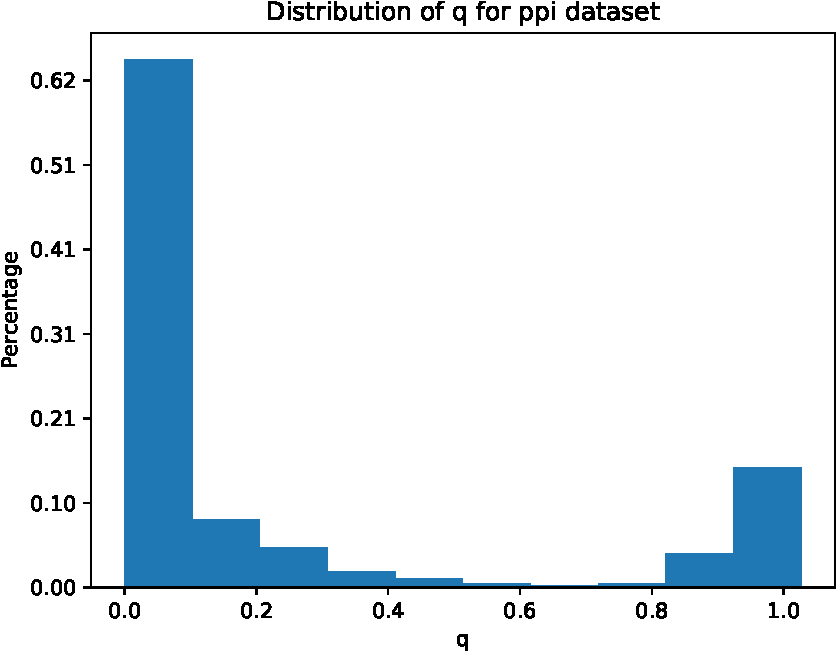
\includegraphics[width=0.245\textwidth]{cs699/fig/ppi.pdf}
    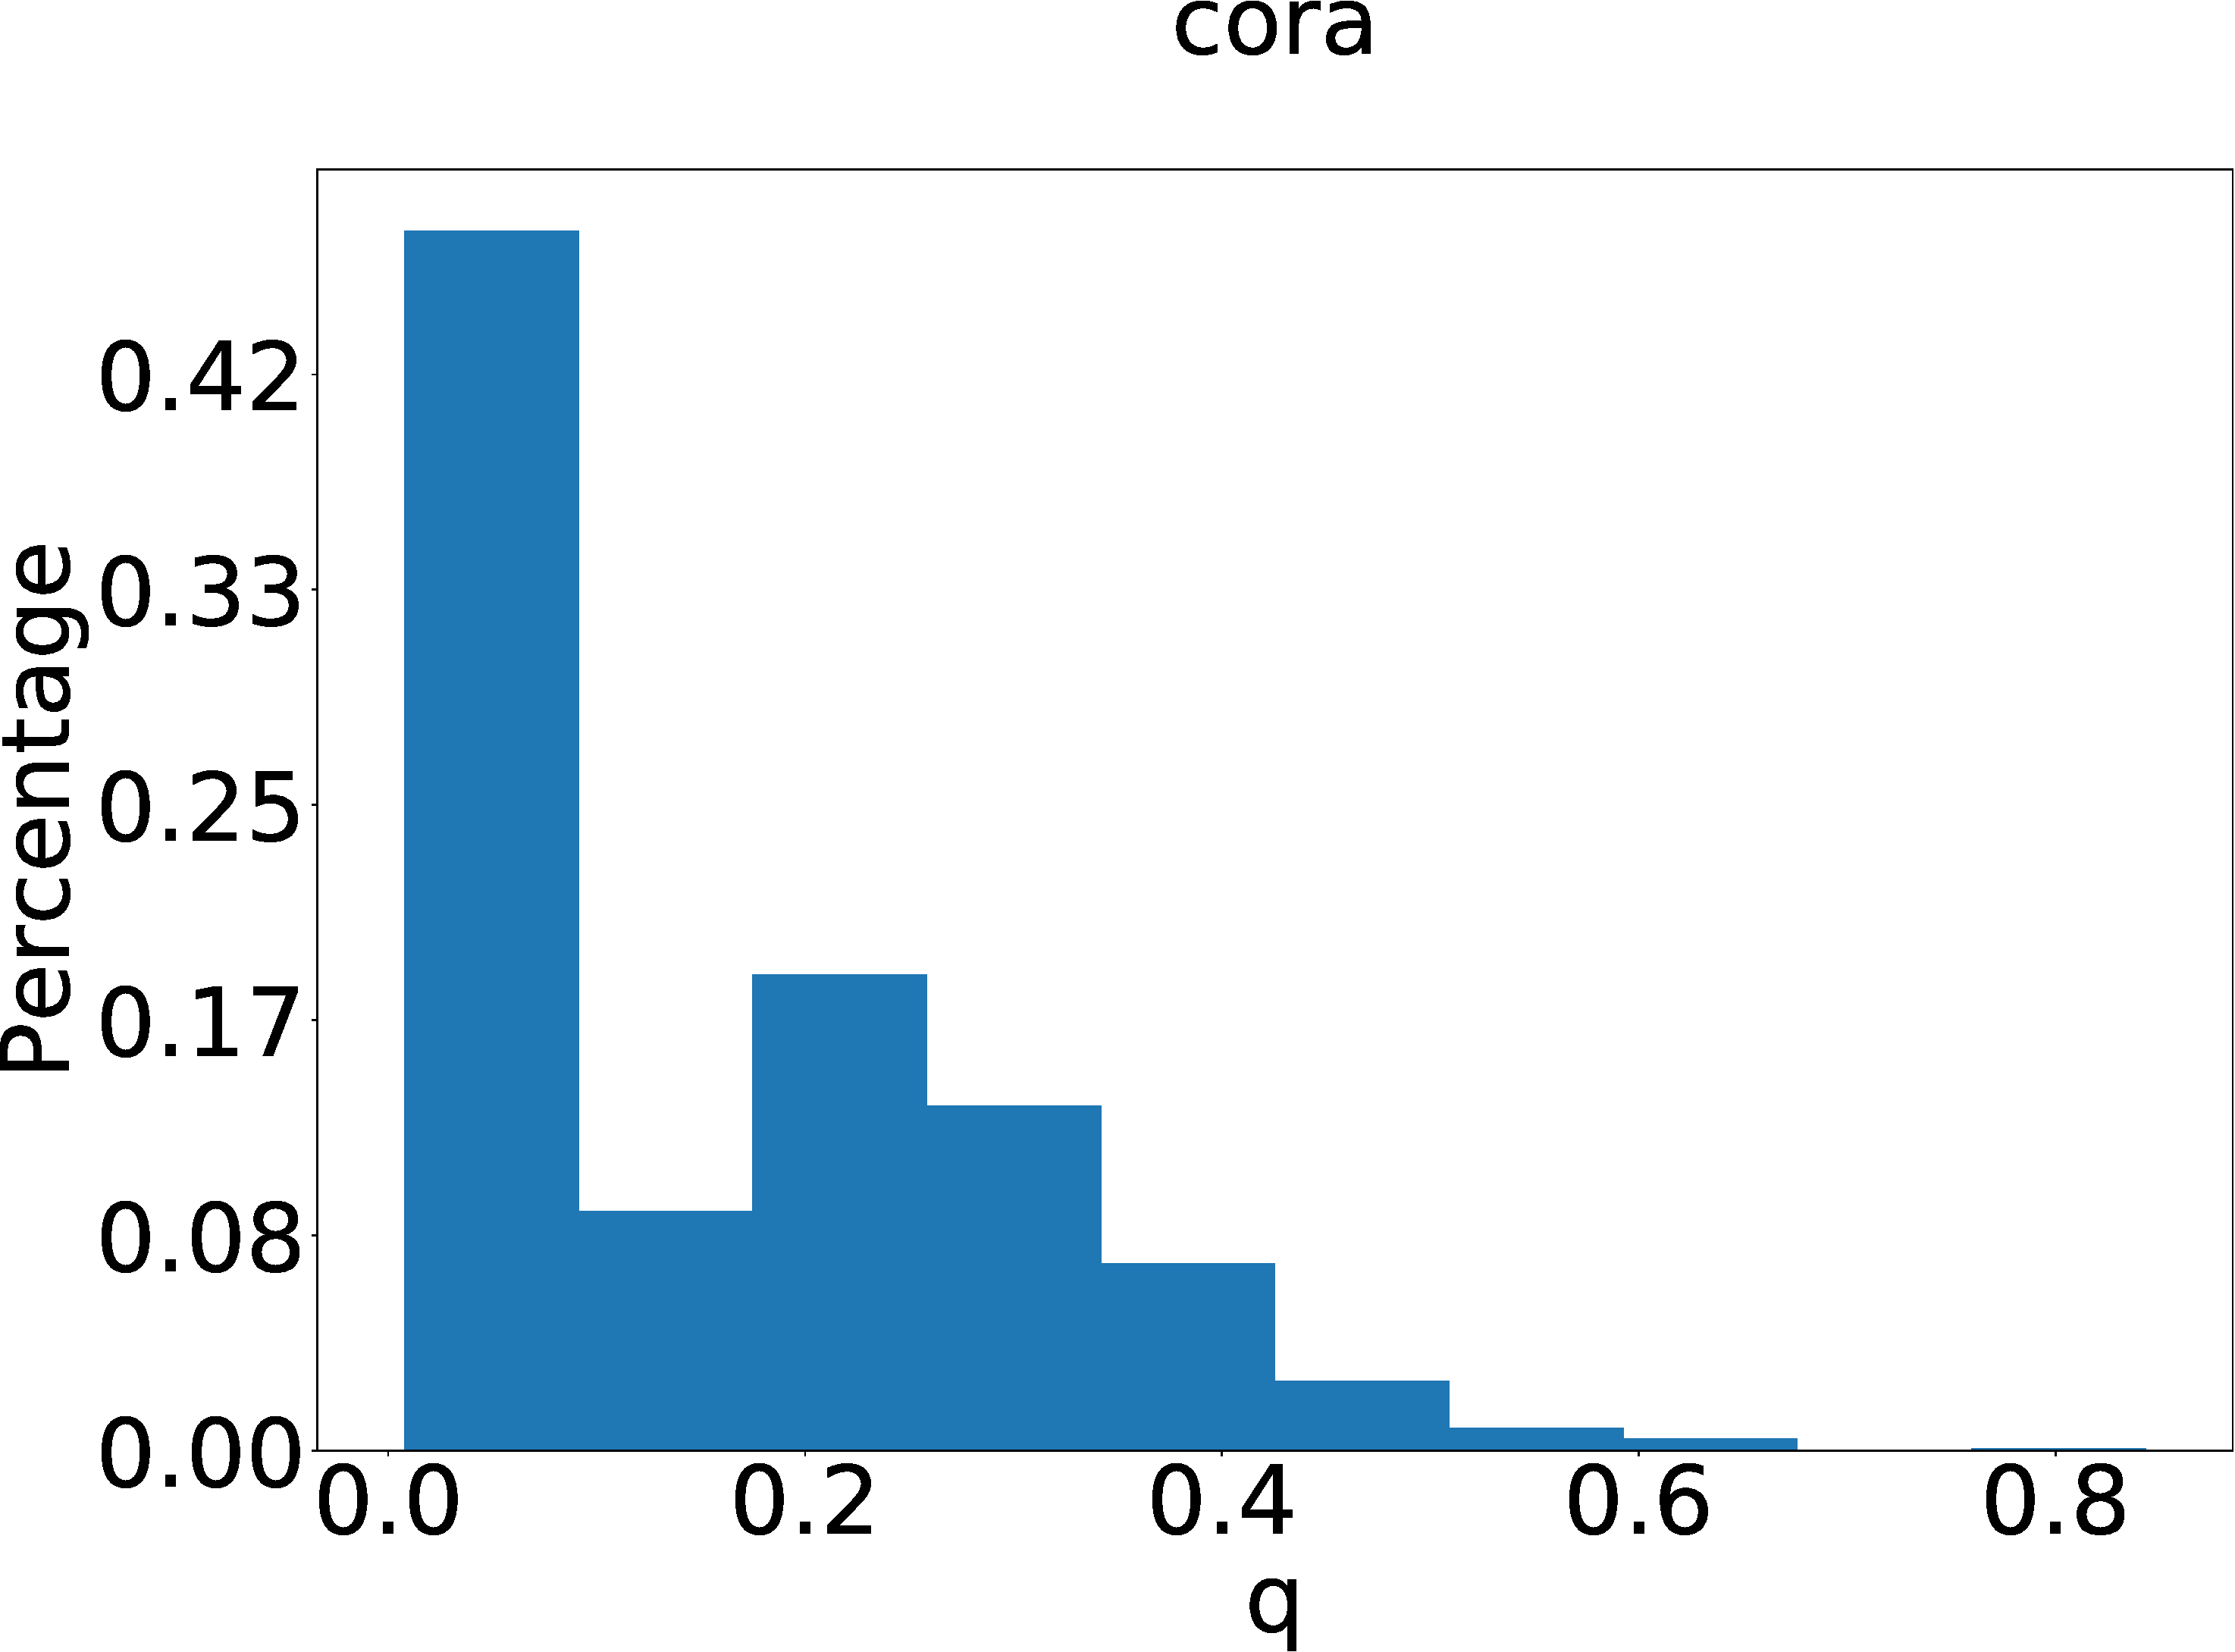
\includegraphics[width=0.245\textwidth]{cs699/fig/cora.pdf}
    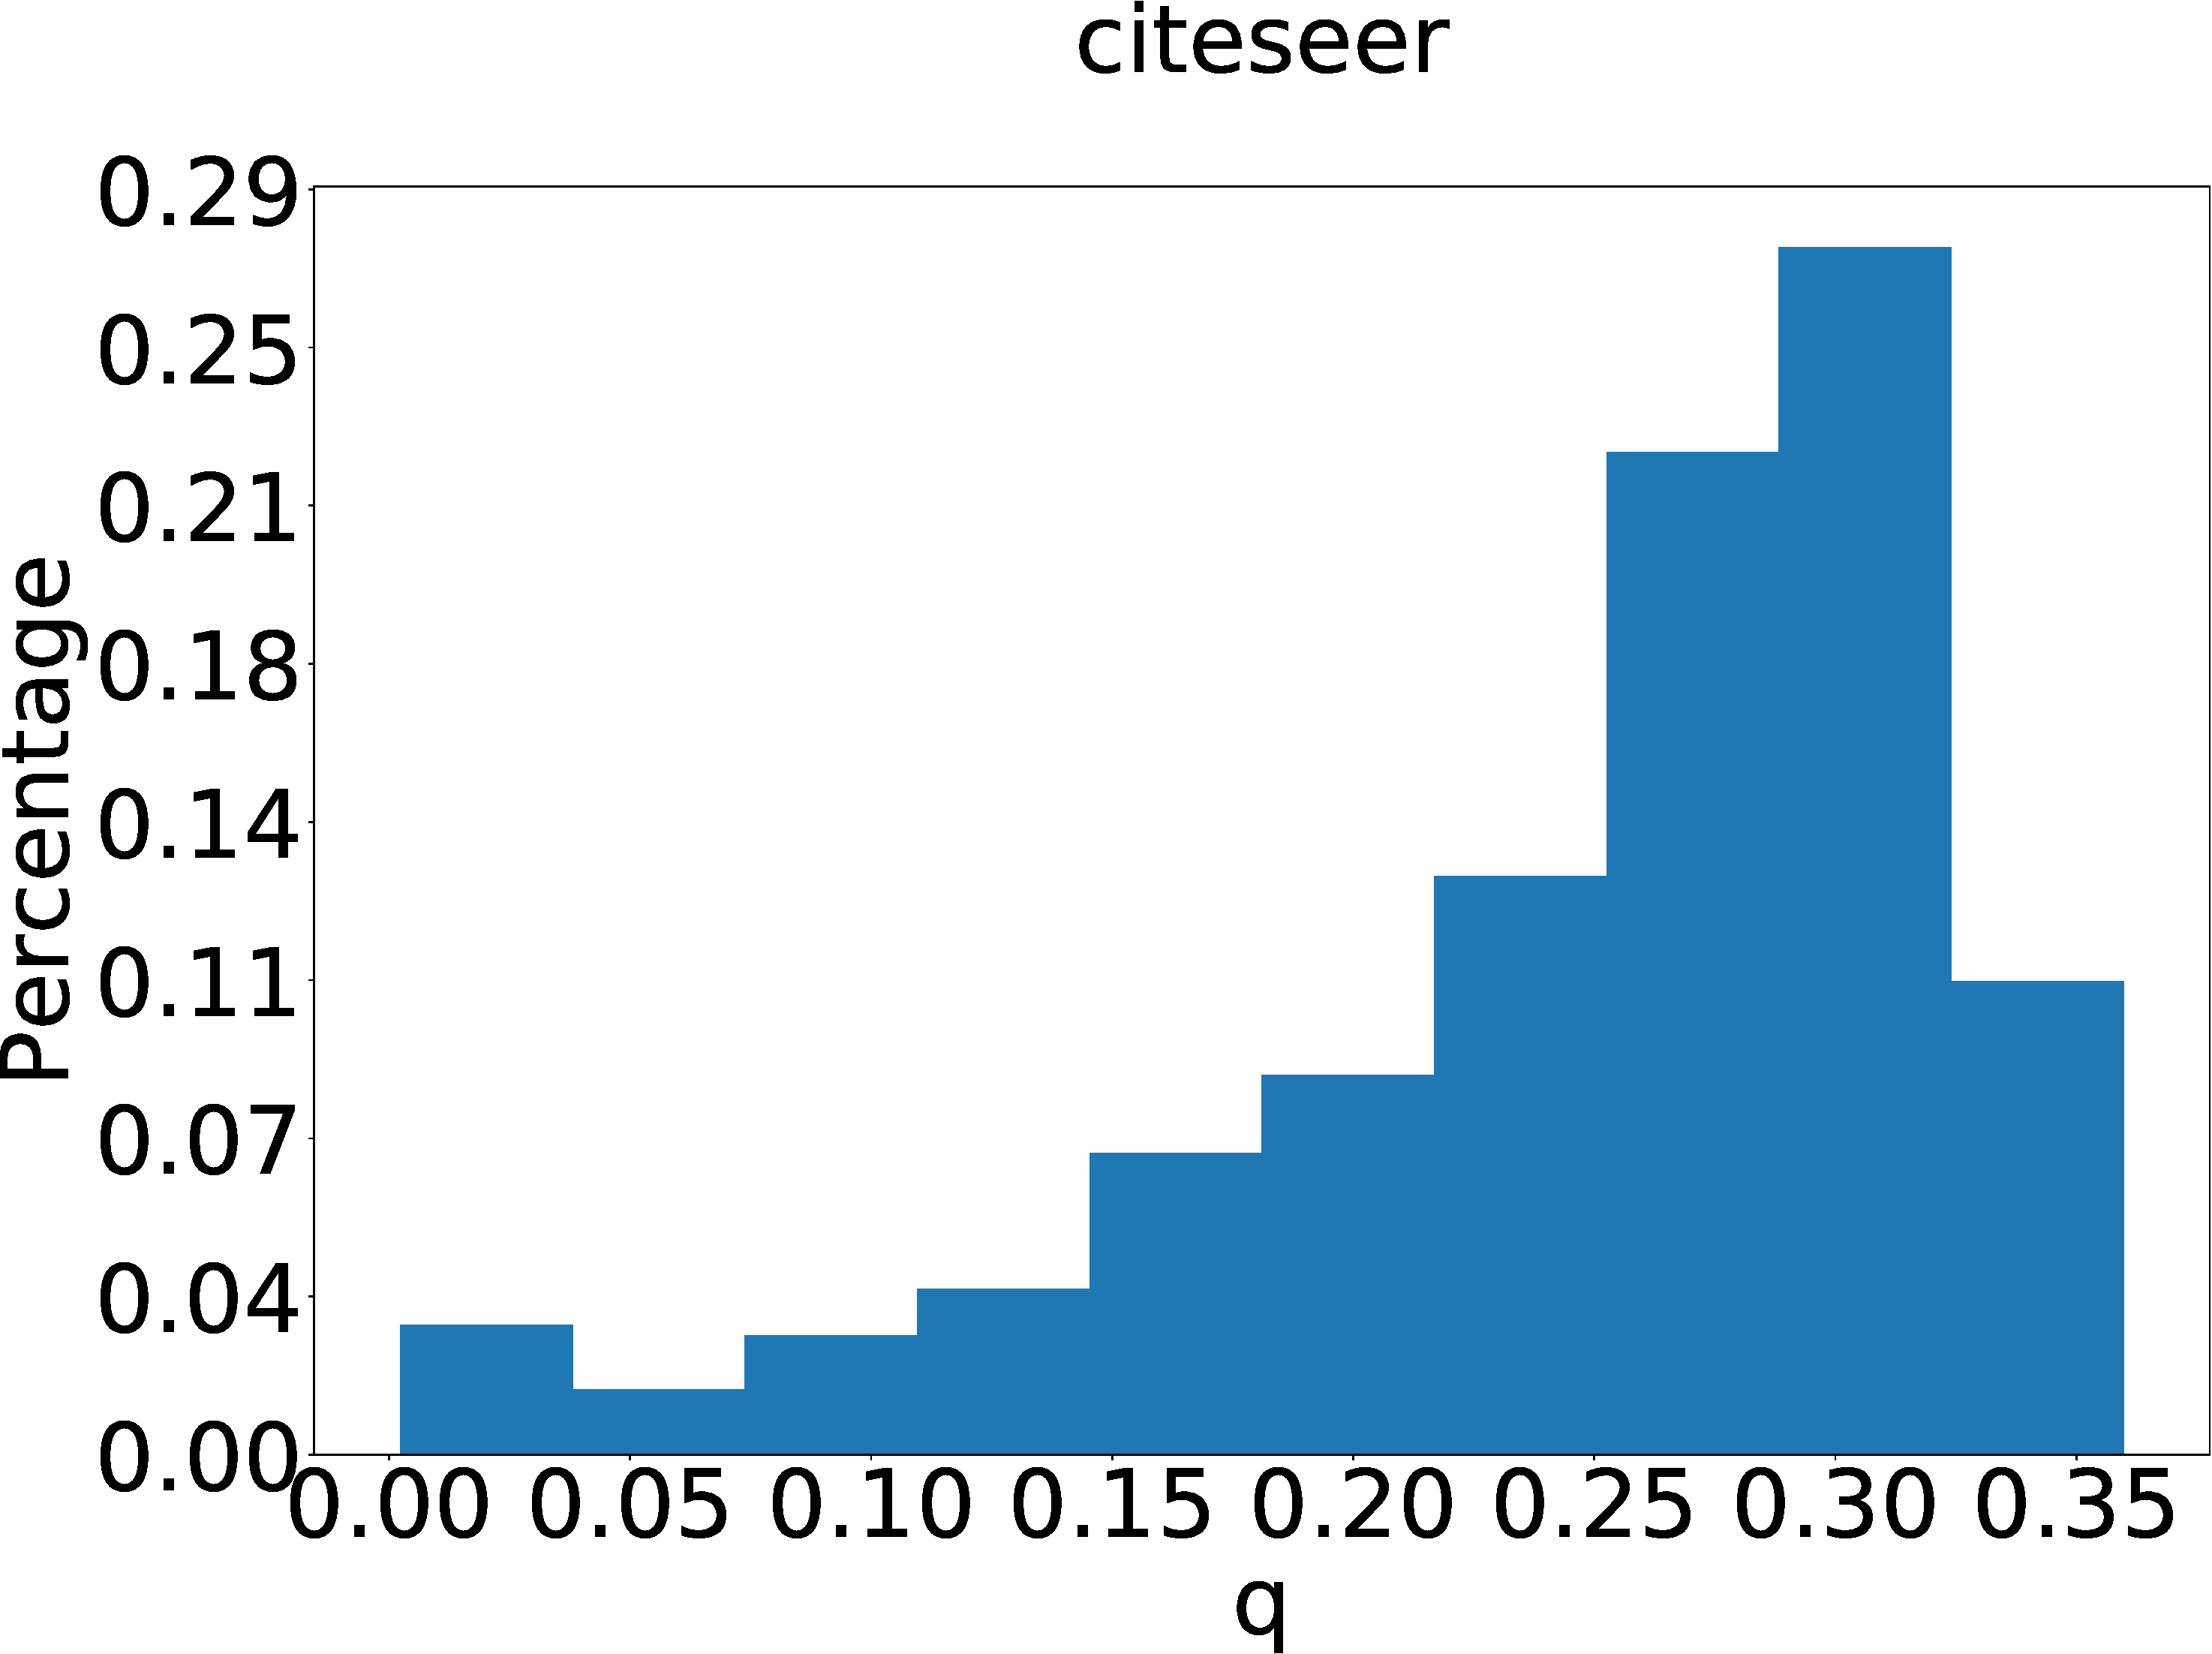
\includegraphics[width=0.245\textwidth]{cs699/fig/citeseer.pdf}\\
    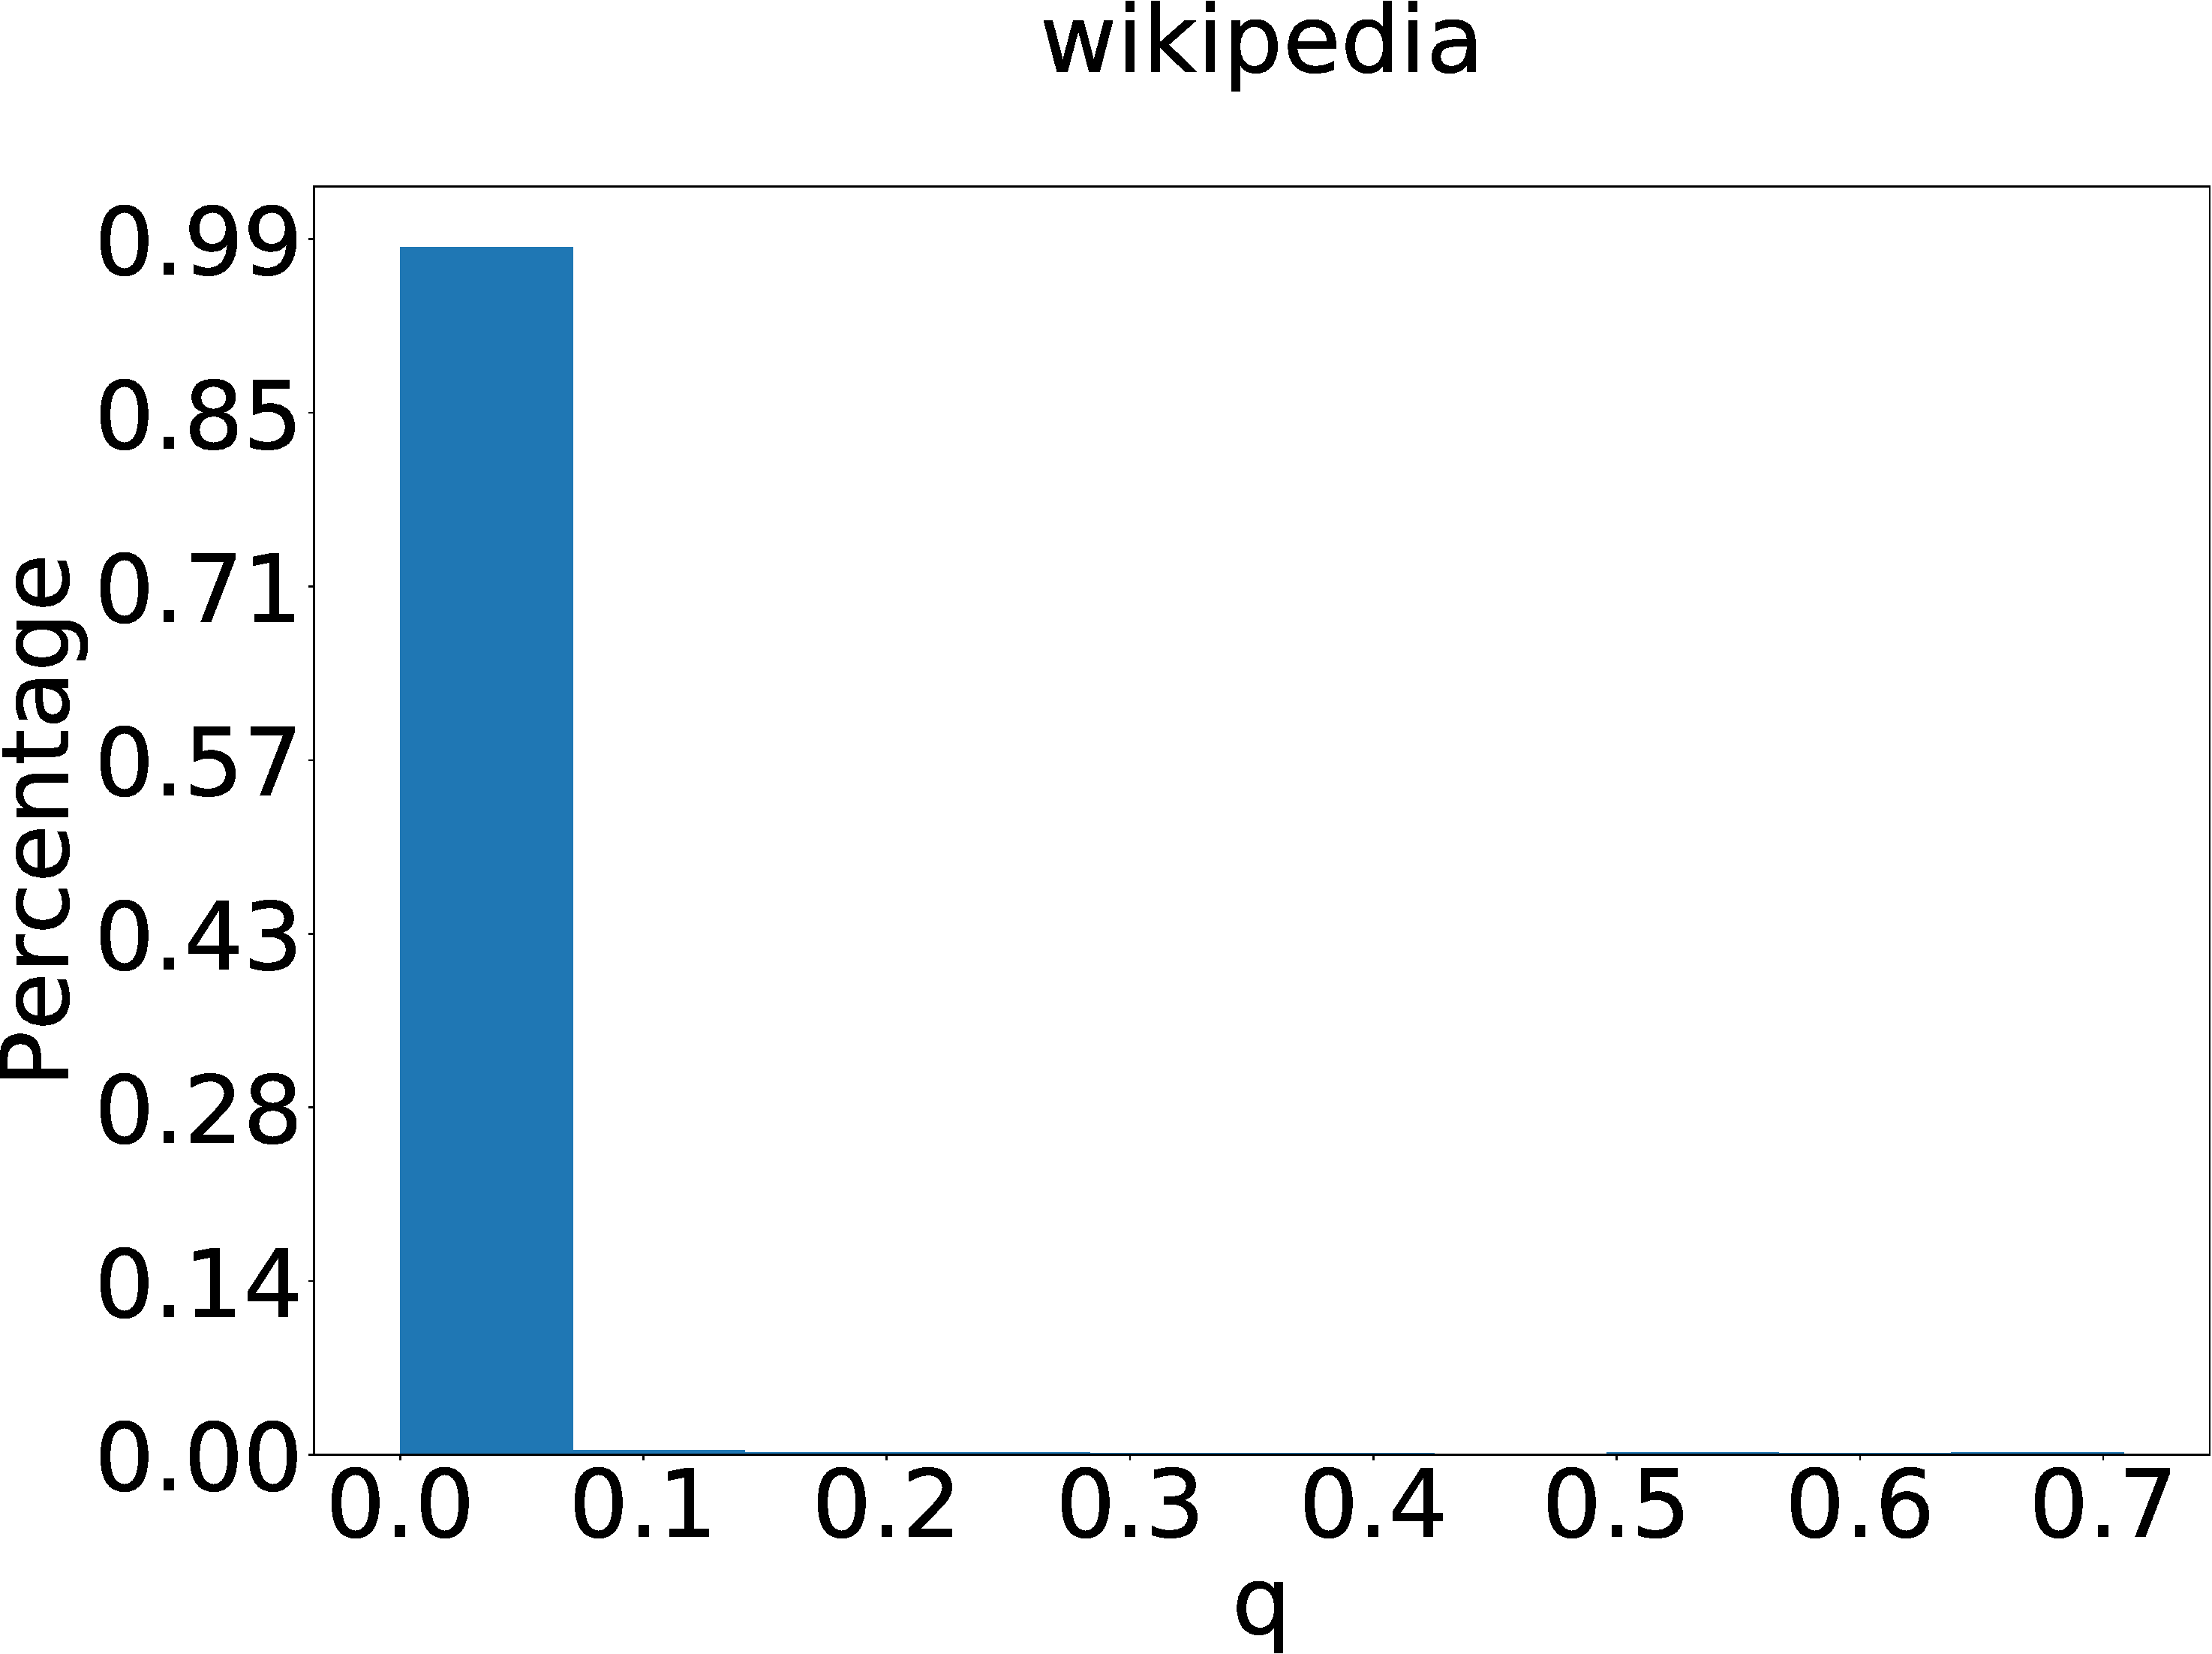
\includegraphics[width=0.245\textwidth]{cs699/fig/wikipedia.pdf}
    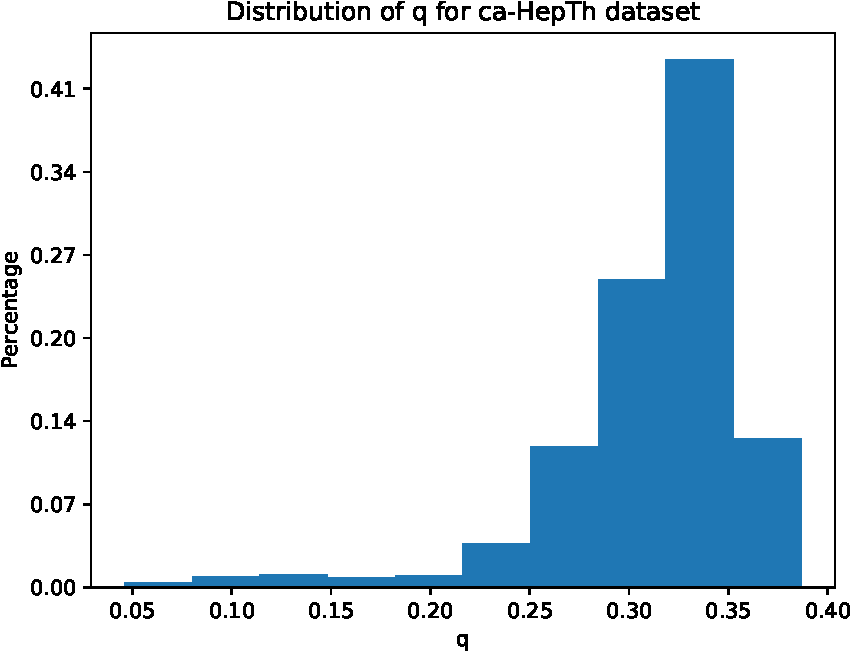
\includegraphics[width=0.245\textwidth]{cs699/fig/ca-HepTh.pdf}
    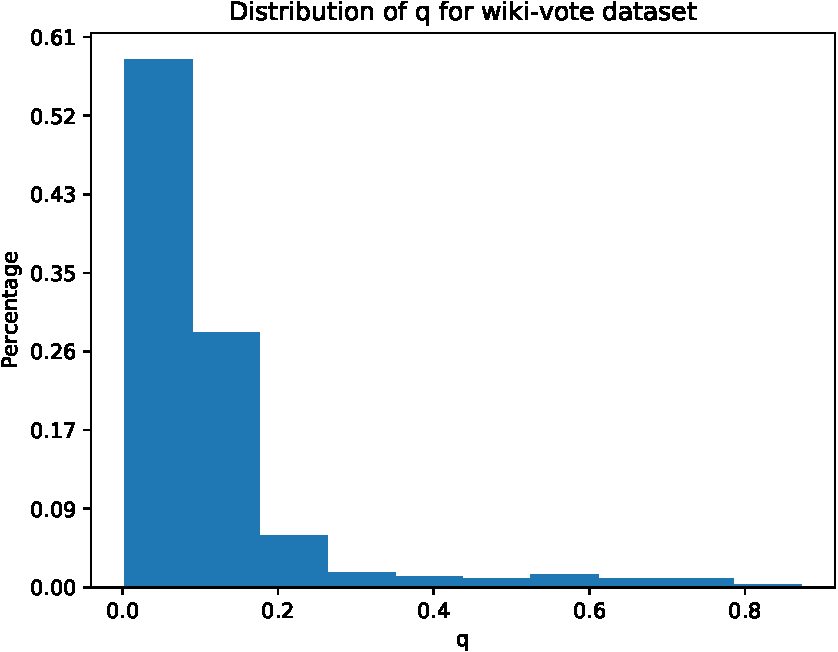
\includegraphics[width=0.245\textwidth]{cs699/fig/wiki-vote.pdf}
    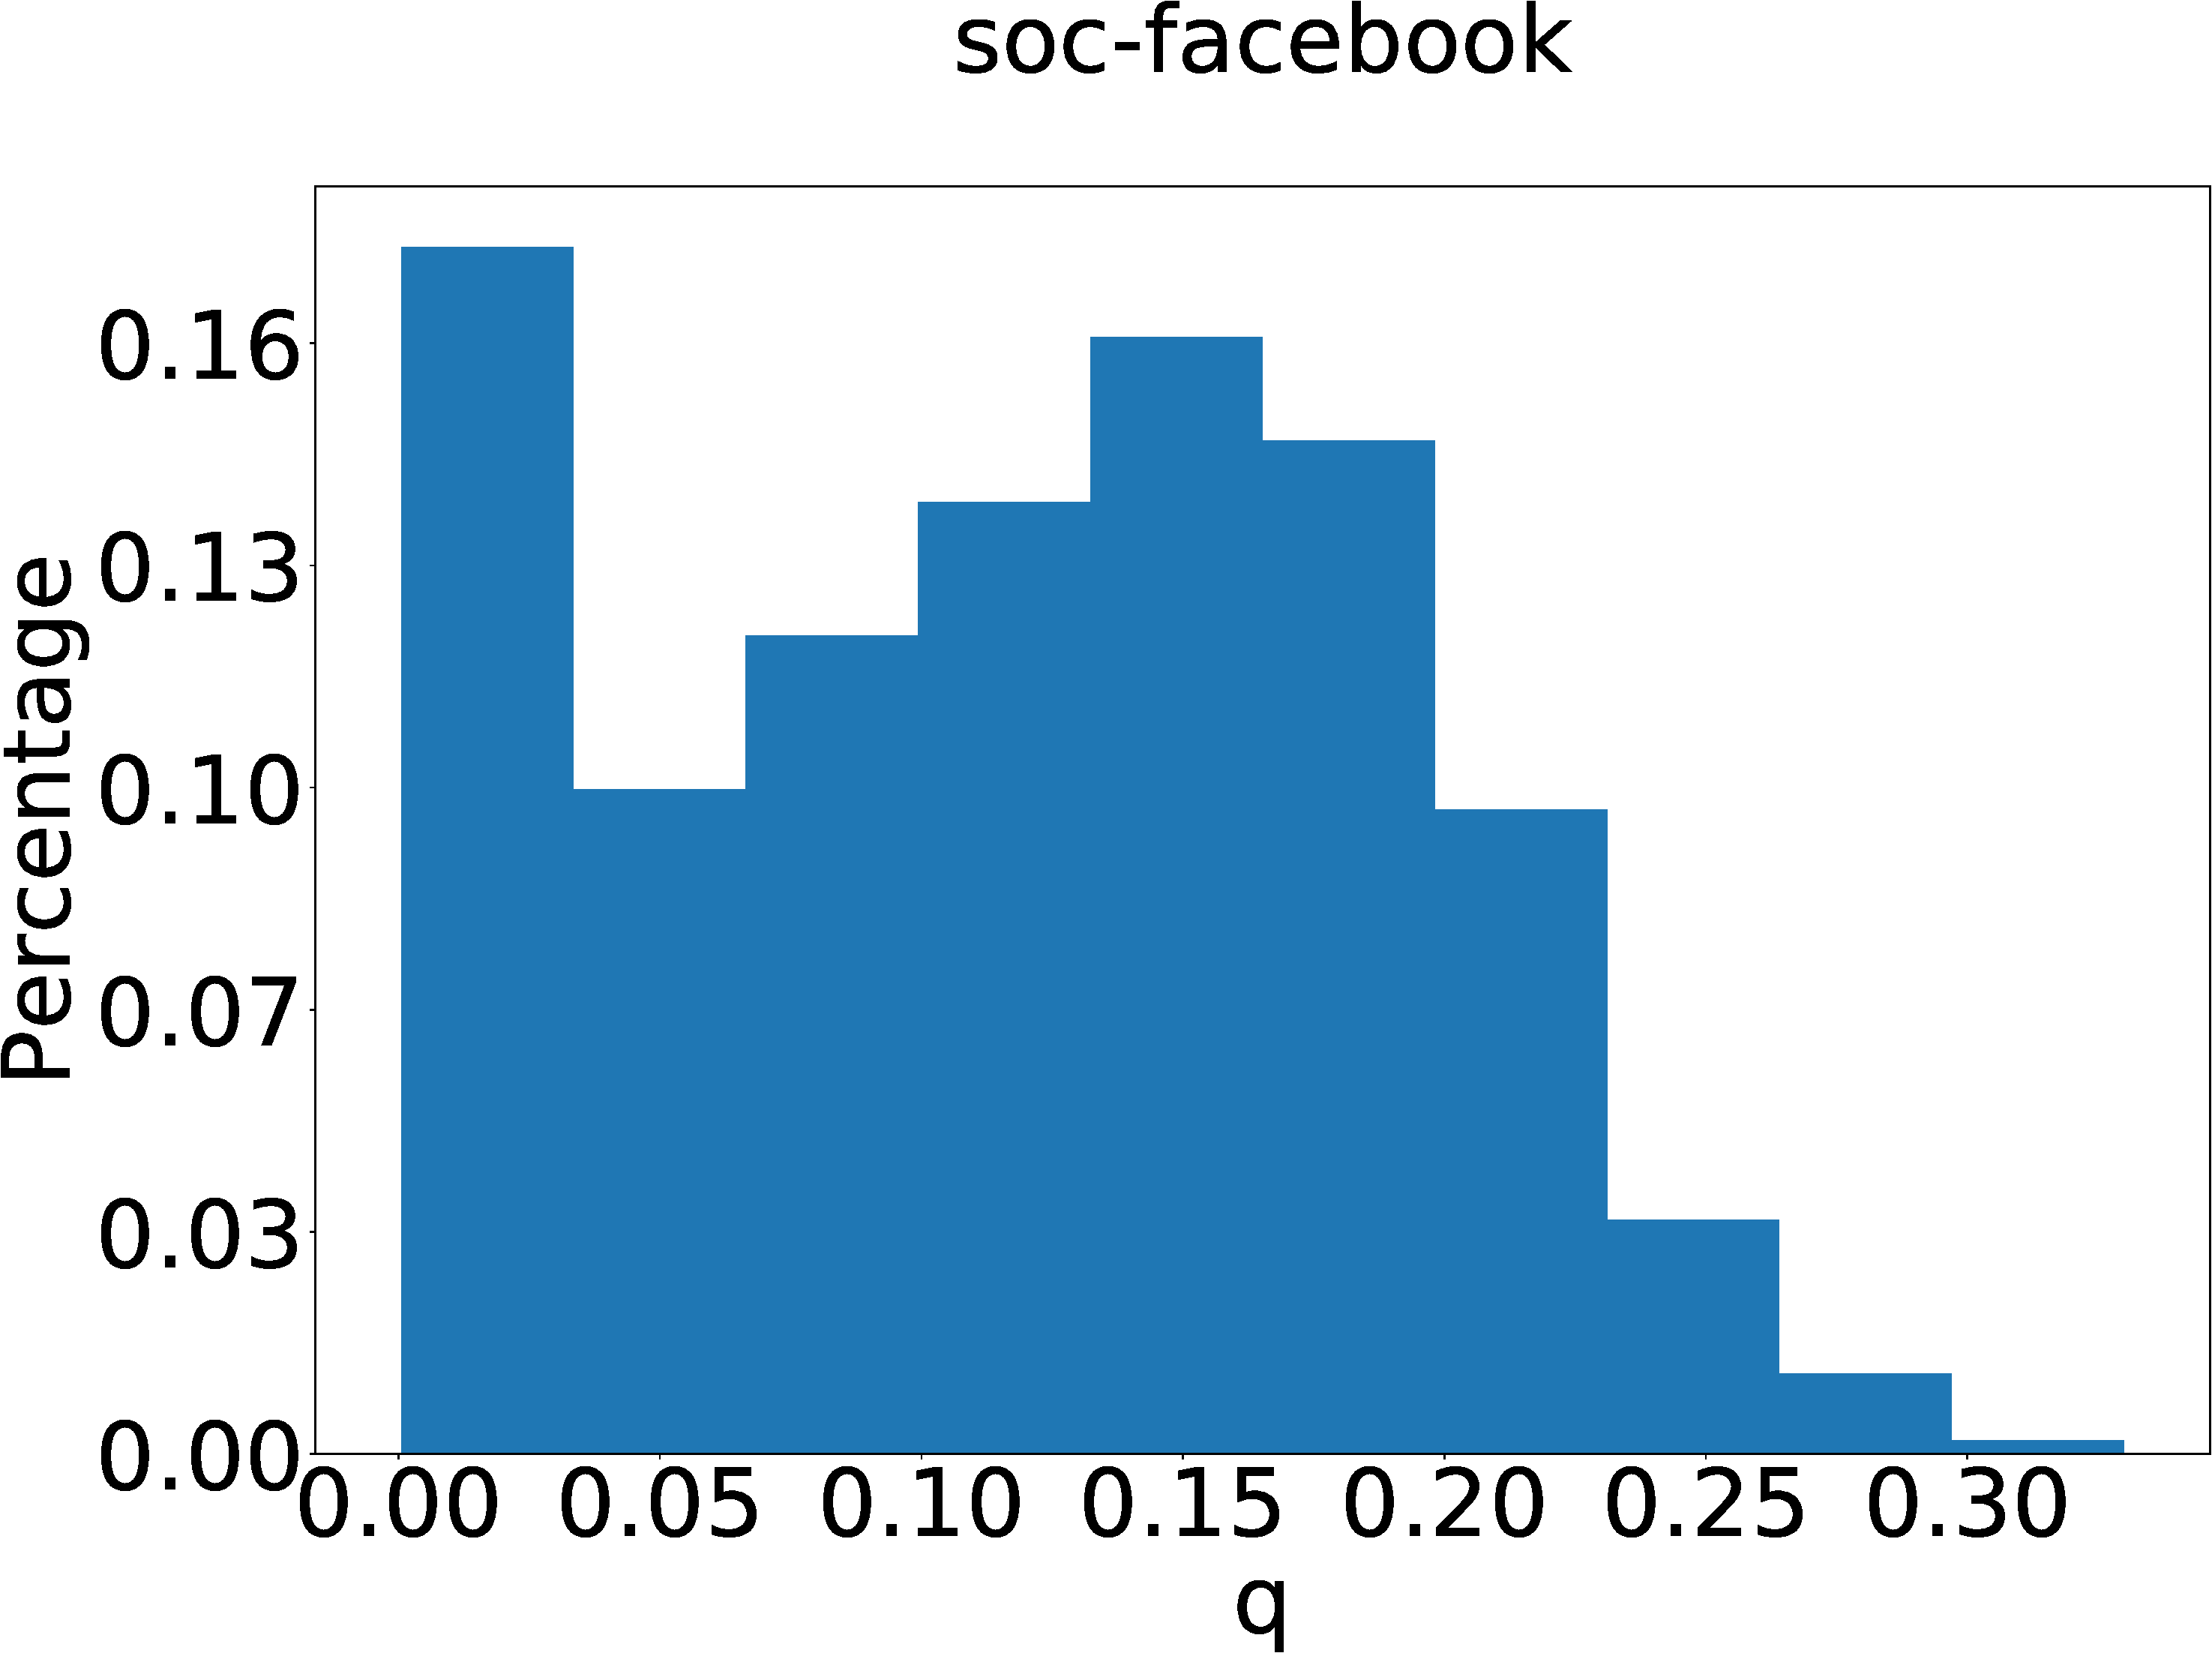
\includegraphics[width=0.245\textwidth]{cs699/fig/soc-facebook.pdf}
    \caption{Distribution of q in different datasets}
    \label{fig:dist_q}
\end{figure}

\begin{table}
\caption{Statistics of q in exponential distribution}
\label{tab:analysis_q}
\centering
\begin{tabular}{ccccccc}
\toprule
Dataset & Min  & Max & Mean & Median & Skewness & Kurtosis \\
\midrule
PPI & 5e-4  & 1.03 & 0.24 & 0.05 & 1.38 & 0.12 \\
Cora & 7e-3  & 0.84 & 0.16 & 0.14 & 0.92 & 0.28 \\
Citeseer & 2e-3  & 0.36  & 0.25 & 0.27 & -1.22 & 1.05 \\
Wikipedia & 2e-5  & 0.71  & 6e-3 & 4e-4 & 10.92 & 126.92 \\
Ca-Hepth & 5e-2  & 0.39  & 0.31 & 0.32 & -2.23 & 6.64 \\
Wikivote & 3e-3  & 0.87  & 0.12 & 0.07 & 2.96 & 9.54\\
Soc-facebook & 5e-4  & 0.33 & 0.12 & 0.12 & 0.03 & -0.92 \\

\bottomrule
\end{tabular}
\end{table}

\begin{figure}
    \centering
    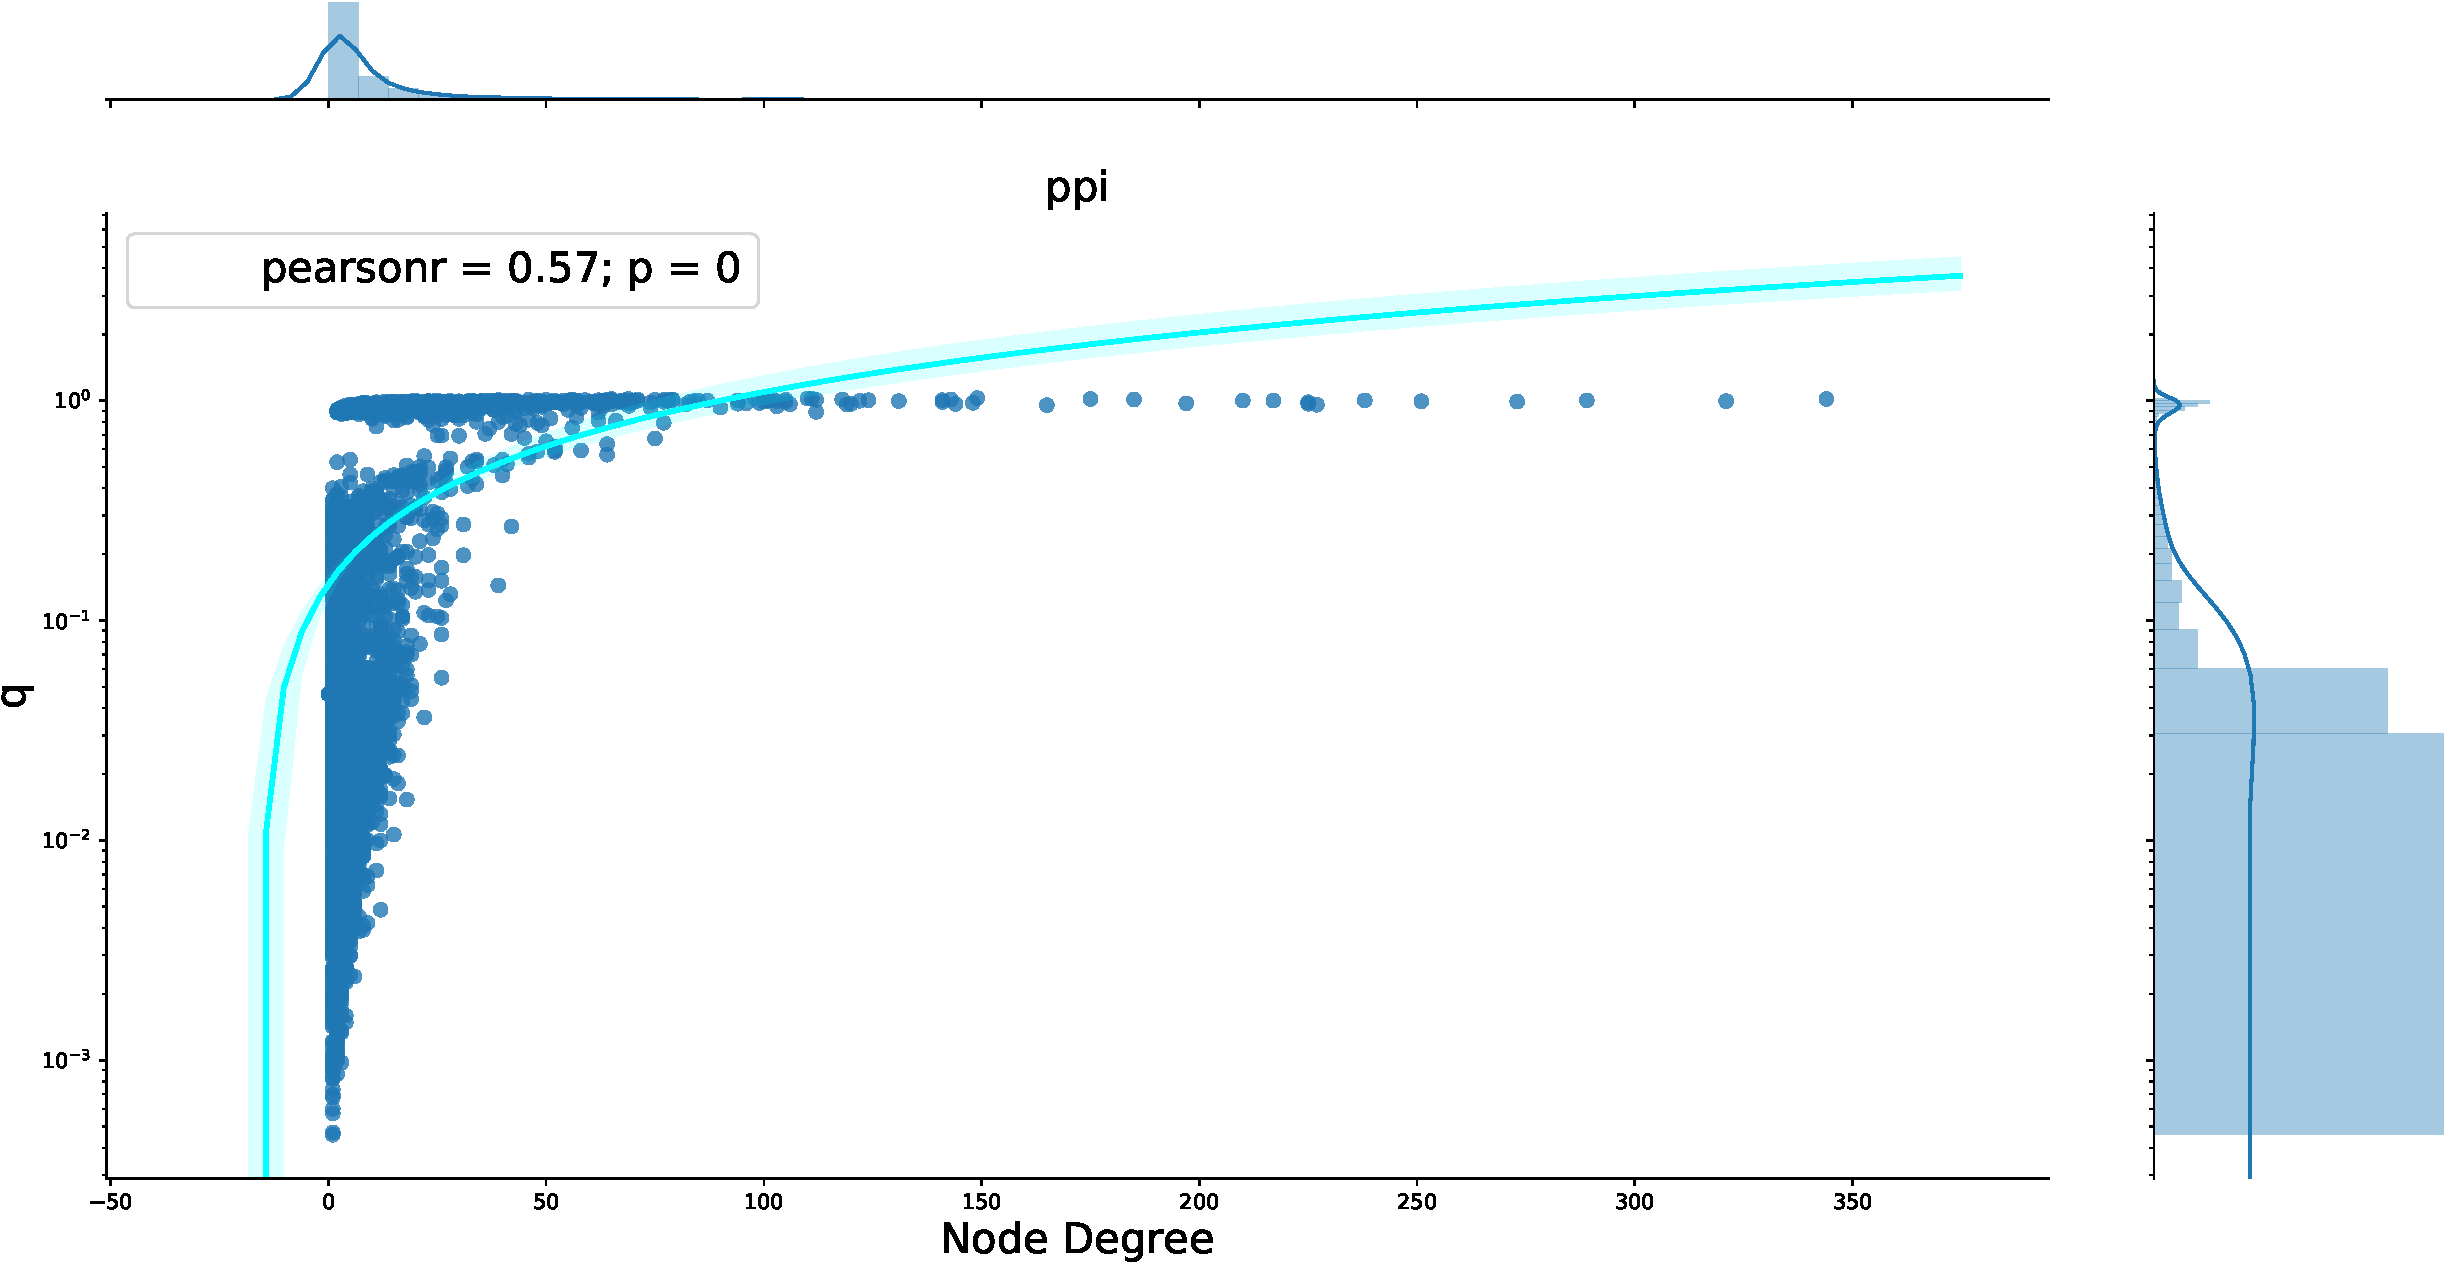
\includegraphics[width=\textwidth]{cs699/fig/degree_q.pdf}
    \caption{Linear regression between node degree and q on PPI dataset with y-axis on logrithmic scale. $R^2$ is 0.57.}
    \label{fig:degree_q}
\end{figure}

% From Fig. \ref{fig:degree_q}, XXX. PPI dataset, y is log scaled. pearsonr = 0.57, p = 0 means it's very likely node degree is correlated with q.

From Figure \ref{fig:degree_q}, we can see a very strong linear correlation between the attention distribution and its degree. Specifically, a higher exponential base $q$ demonstrates a node's more moderate decrease on attention on its further neighbors, which leads to a larger window size. Consequently, the conclusion here is that a hub (with higher degree) is prone to attend to more of its neighbors while more disconnected nodes bear more resemblance to its direct neighbors.

\textbf{Analysis of personalized quadratic distribution.}
Quadratic distribution is more flexible than exponential distribution, which allows a non-monotonic trend of attention weights. We compute the trend by checking the axis of symmetry $\frac{-b}{2a}$ and coefficient $a$. 
From Figure. \ref{fig:dist_mirror}, we found a large portion of node learns a non-monotonic attention distribution, which cannot be captured by exponential distribution. For instance, in Wikipedia dataset, almost all nodes follow a Dec-Inc attention distribution, indicating more attention is placed on neighboring and further away nodes, while the nodes in between are less referred to.

\begin{figure}
    \centering
    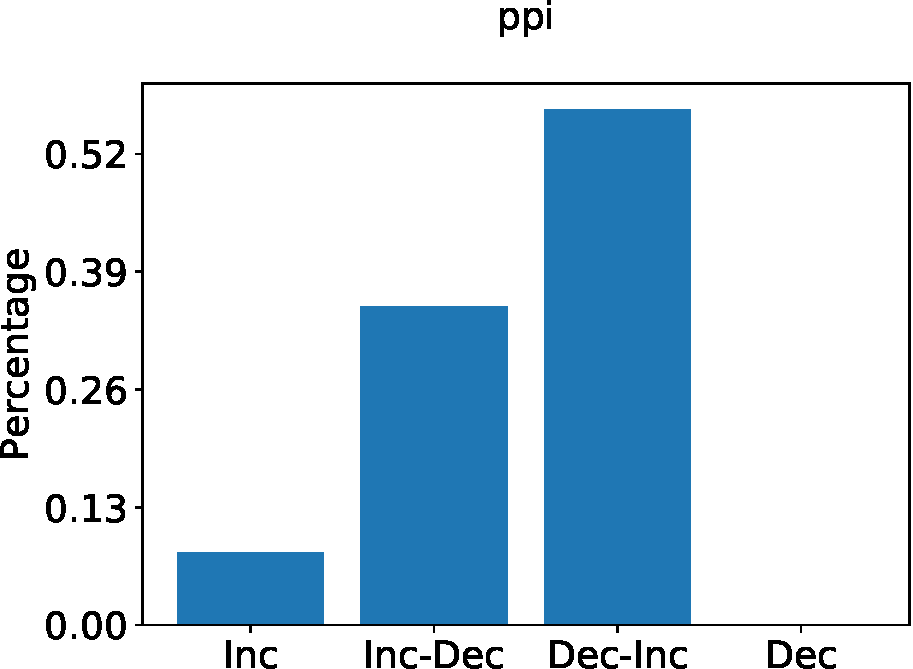
\includegraphics[width=0.245\textwidth]{cs699/fig/ppi_quad.pdf}
    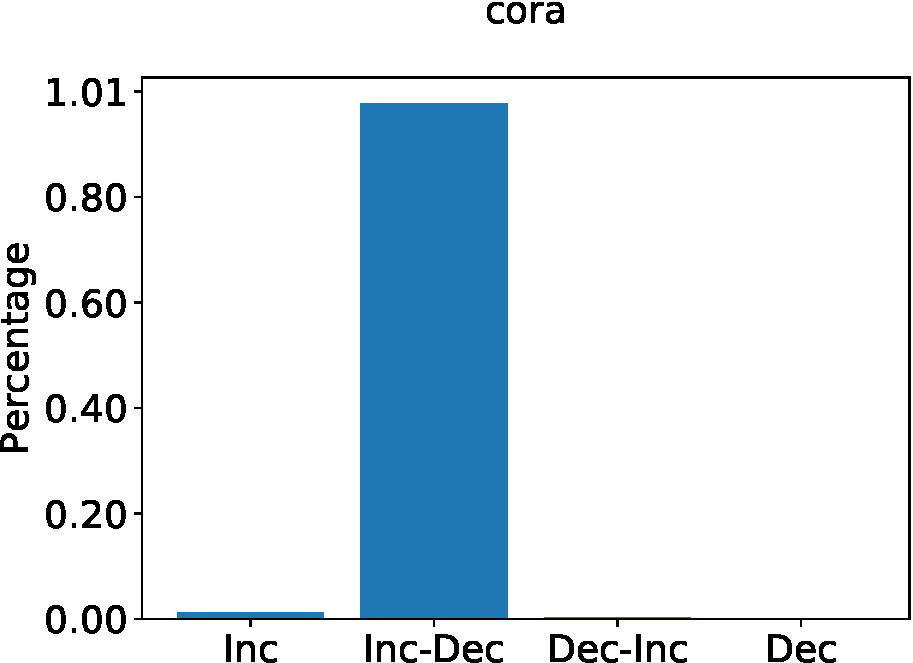
\includegraphics[width=0.245\textwidth]{cs699/fig/cora_quad.pdf}
    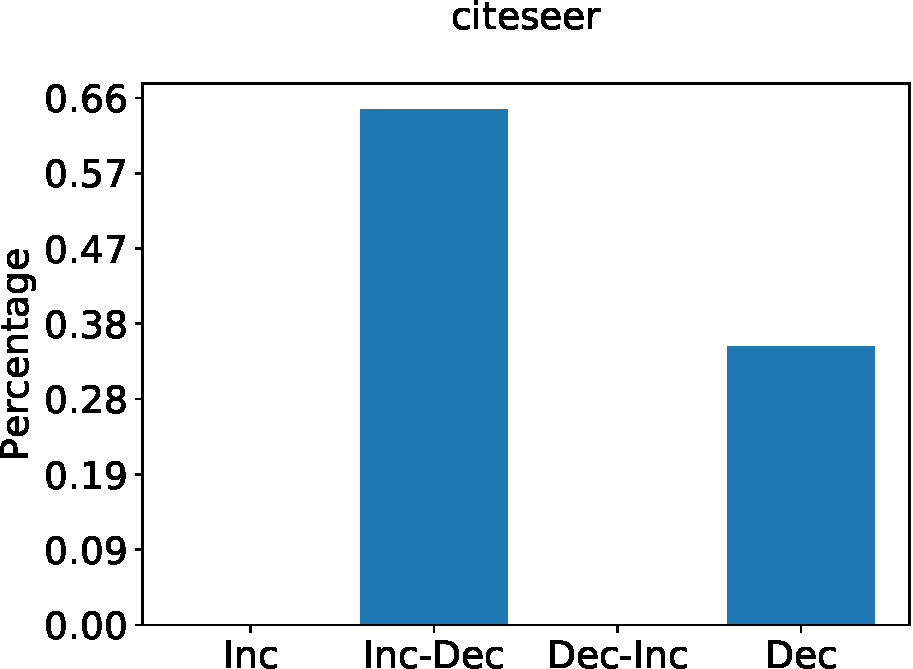
\includegraphics[width=0.245\textwidth]{cs699/fig/citeseer_quad.pdf}\\
    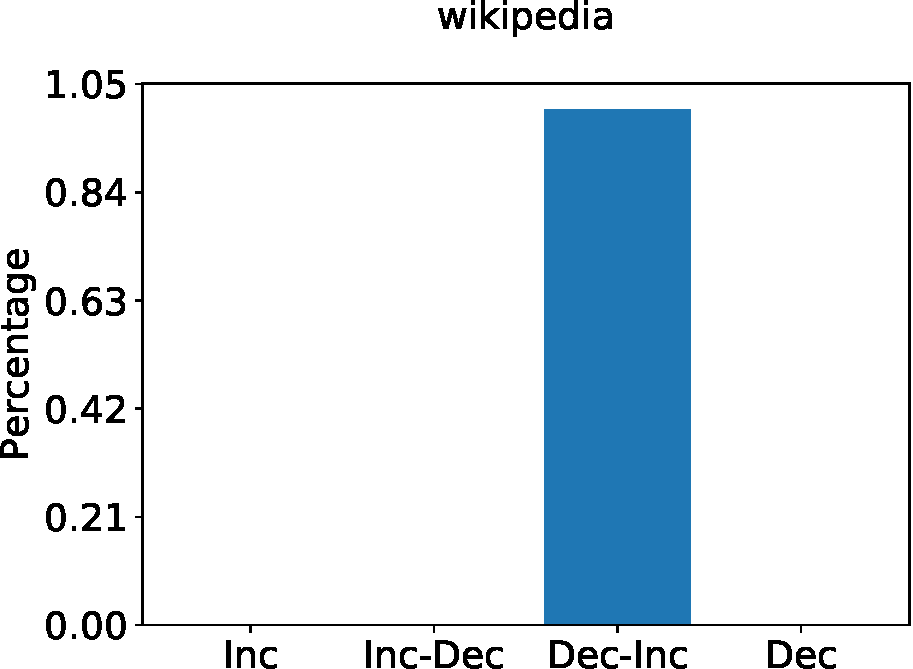
\includegraphics[width=0.245\textwidth]{cs699/fig/wikipedia_quad.pdf}
    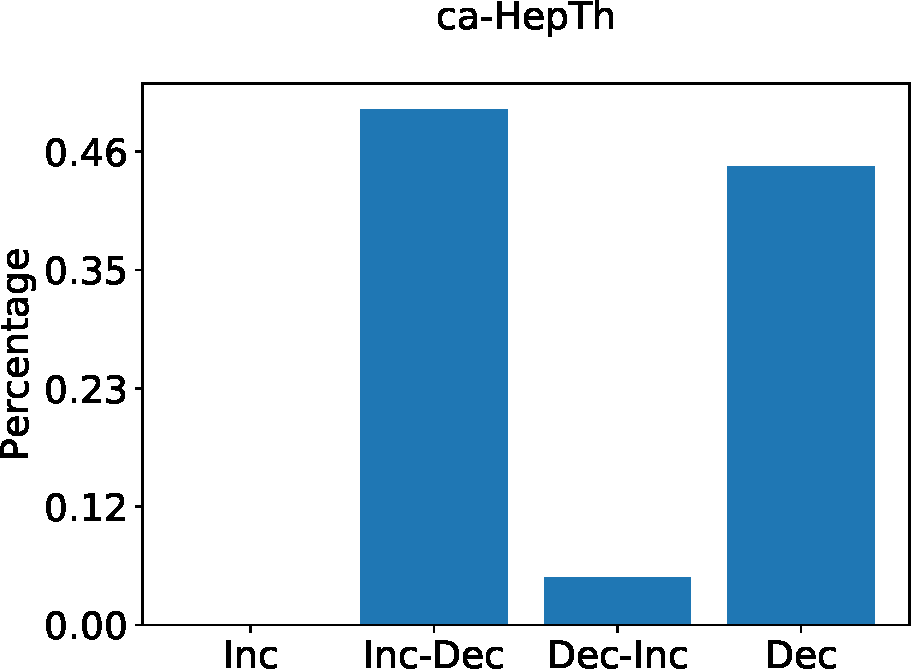
\includegraphics[width=0.245\textwidth]{cs699/fig/ca-HepTh_quad.pdf}
    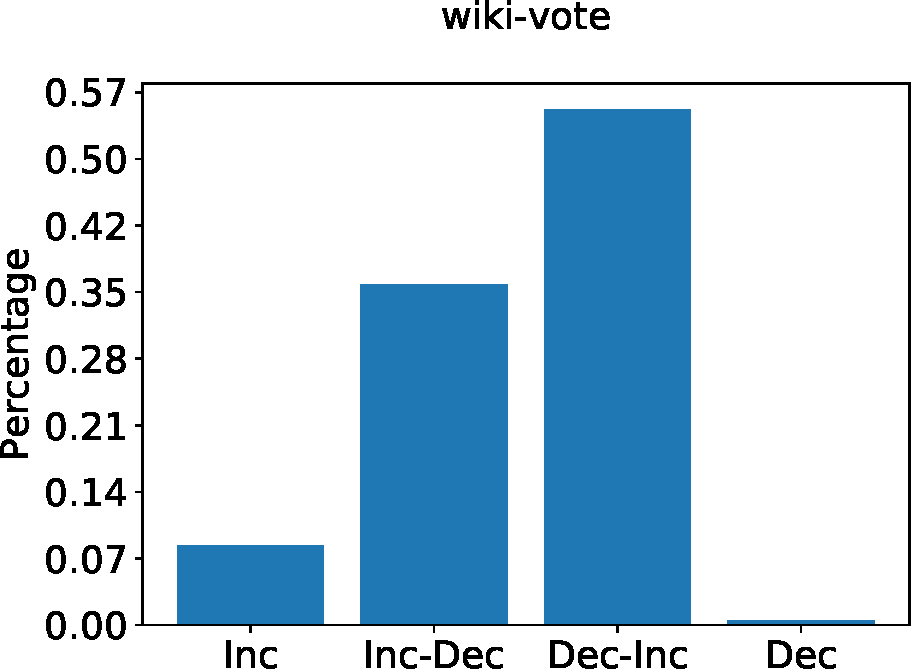
\includegraphics[width=0.245\textwidth]{cs699/fig/wiki-vote_quad.pdf}
    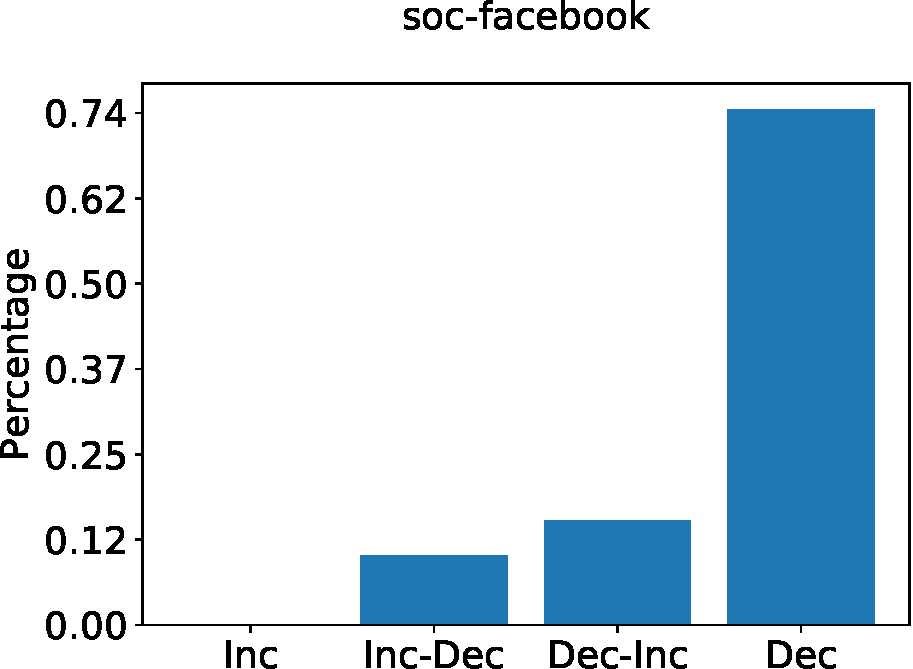
\includegraphics[width=0.245\textwidth]{cs699/fig/soc-facebook_quad.pdf}
    \caption{Distribution of four attention distribution trends captured by quadratic distribution. The four trends are monotonically increasing (Inc), monotonically decreasing (Dec), increasing and decreasing (Inc-Dec), and decreasing and increasing (Dec-Inc.)}
    \label{fig:dist_mirror}
\end{figure}


\section{Conclusions and Future Work}
In this paper, we propose a graph embedding method which extends WatchYourStep by personalizing context distribution for each individual node. We demonstrate the superiority of our method by evaluating the learned embedding on two downstream tasks: link prediction and multi-class node classification. In both tasks, our method outperforms all other compared methods on all benchmark datasets. 

One possible future work is to initialize embedding of each node based on its role in the graph. Another direction of future work is to apply our method to other domains which involve embedding learning such as natural language processing. For example, word embedding can be potentially learned in a personalized way.

% Please read the instructions below carefully and follow them faithfully.

% \subsection{Style}

% Papers to be submitted to NeurIPS 2019 must be prepared according to the
% instructions presented here. Papers may only be up to eight pages long,
% including figures. Additional pages \emph{containing only acknowledgments and/or
%   cited references} are allowed. Papers that exceed eight pages of content
% (ignoring references) will not be reviewed, or in any other way considered for
% presentation at the conference.

% The margins in 2019 are the same as since 2007, which allow for $\sim$$15\%$
% more words in the paper compared to earlier years.

% Authors are required to use the NeurIPS \LaTeX{} style files obtainable at the
% NeurIPS website as indicated below. Please make sure you use the current files
% and not previous versions. Tweaking the style files may be grounds for
% rejection.

% \subsection{Retrieval of style files}

% The style files for NeurIPS and other conference information are available on
% the World Wide Web at
% \begin{center}
%   \url{http://www.neurips.cc/}
% \end{center}
% The file \verb+neurips_2019.pdf+ contains these instructions and illustrates the
% various formatting requirements your NeurIPS paper must satisfy.

% The only supported style file for NeurIPS 2019 is \verb+neurips_2019.sty+,
% rewritten for \LaTeXe{}.  \textbf{Previous style files for \LaTeX{} 2.09,
%   Microsoft Word, and RTF are no longer supported!}

% The \LaTeX{} style file contains three optional arguments: \verb+final+, which
% creates a camera-ready copy, \verb+preprint+, which creates a preprint for
% submission to, e.g., arXiv, and \verb+nonatbib+, which will not load the
% \verb+natbib+ package for you in case of package clash.

% \paragraph{Preprint option}
% If you wish to post a preprint of your work online, e.g., on arXiv, using the
% NeurIPS style, please use the \verb+preprint+ option. This will create a
% nonanonymized version of your work with the text ``Preprint. Work in progress.''
% in the footer. This version may be distributed as you see fit. Please \textbf{do
%   not} use the \verb+final+ option, which should \textbf{only} be used for
% papers accepted to NeurIPS.

% At submission time, please omit the \verb+final+ and \verb+preprint+
% options. This will anonymize your submission and add line numbers to aid
% review. Please do \emph{not} refer to these line numbers in your paper as they
% will be removed during generation of camera-ready copies.

% The file \verb+neurips_2019.tex+ may be used as a ``shell'' for writing your
% paper. All you have to do is replace the author, title, abstract, and text of
% the paper with your own.

% The formatting instructions contained in these style files are summarized in
% Sections \ref{gen_inst}, \ref{headings}, and \ref{others} below.

% \section{General formatting instructions}
% \label{gen_inst}

% The text must be confined within a rectangle 5.5~inches (33~picas) wide and
% 9~inches (54~picas) long. The left margin is 1.5~inch (9~picas).  Use 10~point
% type with a vertical spacing (leading) of 11~points.  Times New Roman is the
% preferred typeface throughout, and will be selected for you by default.
% Paragraphs are separated by \nicefrac{1}{2}~line space (5.5 points), with no
% indentation.

% The paper title should be 17~point, initial caps/lower case, bold, centered
% between two horizontal rules. The top rule should be 4~points thick and the
% bottom rule should be 1~point thick. Allow \nicefrac{1}{4}~inch space above and
% below the title to rules. All pages should start at 1~inch (6~picas) from the
% top of the page.

% For the final version, authors' names are set in boldface, and each name is
% centered above the corresponding address. The lead author's name is to be listed
% first (left-most), and the co-authors' names (if different address) are set to
% follow. If there is only one co-author, list both author and co-author side by
% side.

% Please pay special attention to the instructions in Section \ref{others}
% regarding figures, tables, acknowledgments, and references.

% \section{Headings: first level}
% \label{headings}

% All headings should be lower case (except for first word and proper nouns),
% flush left, and bold.

% First-level headings should be in 12-point type.

% \subsection{Headings: second level}

% Second-level headings should be in 10-point type.

% \subsubsection{Headings: third level}

% Third-level headings should be in 10-point type.

% \paragraph{Paragraphs}

% There is also a \verb+\paragraph+ command available, which sets the heading in
% bold, flush left, and inline with the text, with the heading followed by 1\,em
% of space.

% \section{Citations, figures, tables, references}
% \label{others}

% These instructions apply to everyone.

% \subsection{Citations within the text}

% The \verb+natbib+ package will be loaded for you by default.  Citations may be
% author/year or numeric, as long as you maintain internal consistency.  As to the
% format of the references themselves, any style is acceptable as long as it is
% used consistently.

% The documentation for \verb+natbib+ may be found at
% \begin{center}
%   \url{http://mirrors.ctan.org/macros/latex/contrib/natbib/natnotes.pdf}
% \end{center}
% Of note is the command \verb+\citet+, which produces citations appropriate for
% use in inline text.  For example,
% \begin{verbatim}
%   \citet{hasselmo} investigated\dots
% \end{verbatim}
% produces
% \begin{quote}
%   Hasselmo, et al.\ (1995) investigated\dots
% \end{quote}

% If you wish to load the \verb+natbib+ package with options, you may add the
% following before loading the \verb+neurips_2019+ package:
% \begin{verbatim}
%   \PassOptionsToPackage{options}{natbib}
% \end{verbatim}

% If \verb+natbib+ clashes with another package you load, you can add the optional
% argument \verb+nonatbib+ when loading the style file:
% \begin{verbatim}
%   \usepackage[nonatbib]{neurips_2019}
% \end{verbatim}

% As submission is double blind, refer to your own published work in the third
% person. That is, use ``In the previous work of Jones et al.\ [4],'' not ``In our
% previous work [4].'' If you cite your other papers that are not widely available
% (e.g., a journal paper under review), use anonymous author names in the
% citation, e.g., an author of the form ``A.\ Anonymous.''

% \subsection{Footnotes}

% Footnotes should be used sparingly.  If you do require a footnote, indicate
% footnotes with a number\footnote{Sample of the first footnote.} in the
% text. Place the footnotes at the bottom of the page on which they appear.
% Precede the footnote with a horizontal rule of 2~inches (12~picas).

% Note that footnotes are properly typeset \emph{after} punctuation
% marks.\footnote{As in this example.}

% \subsection{Figures}

% \begin{figure}
%   \centering
%   \fbox{\rule[-.5cm]{0cm}{4cm} \rule[-.5cm]{4cm}{0cm}}
%   \caption{Sample figure caption.}
% \end{figure}

% All artwork must be neat, clean, and legible. Lines should be dark enough for
% purposes of reproduction. The figure number and caption always appear after the
% figure. Place one line space before the figure caption and one line space after
% the figure. The figure caption should be lower case (except for first word and
% proper nouns); figures are numbered consecutively.

% You may use color figures.  However, it is best for the figure captions and the
% paper body to be legible if the paper is printed in either black/white or in
% color.

% \subsection{Tables}

% All tables must be centered, neat, clean and legible.  The table number and
% title always appear before the table.  See Table~\ref{sample-table}.

% Place one line space before the table title, one line space after the
% table title, and one line space after the table. The table title must
% be lower case (except for first word and proper nouns); tables are
% numbered consecutively.

% Note that publication-quality tables \emph{do not contain vertical rules.} We
% strongly suggest the use of the \verb+booktabs+ package, which allows for
% typesetting high-quality, professional tables:
% \begin{center}
%   \url{https://www.ctan.org/pkg/booktabs}
% \end{center}
% This package was used to typeset Table~\ref{sample-table}.

% \begin{table}
%   \caption{Sample table title}
%   \label{sample-table}
%   \centering
%   \begin{tabular}{lll}
%     \toprule
%     \multicolumn{2}{c}{Part}                   \\
%     \cmidrule(r){1-2}
%     Name     & Description     & Size ($\mu$m) \\
%     \midrule
%     Dendrite & Input terminal  & $\sim$100     \\
%     Axon     & Output terminal & $\sim$10      \\
%     Soma     & Cell body       & up to $10^6$  \\
%     \bottomrule
%   \end{tabular}
% \end{table}

% \section{Final instructions}

% Do not change any aspects of the formatting parameters in the style files.  In
% particular, do not modify the width or length of the rectangle the text should
% fit into, and do not change font sizes (except perhaps in the
% \textbf{References} section; see below). Please note that pages should be
% numbered.

% \section{Preparing PDF files}

% Please prepare submission files with paper size ``US Letter,'' and not, for
% example, ``A4.''

% Fonts were the main cause of problems in the past years. Your PDF file must only
% contain Type 1 or Embedded TrueType fonts. Here are a few instructions to
% achieve this.

% \begin{itemize}

% \item You should directly generate PDF files using \verb+pdflatex+.

% \item You can check which fonts a PDF files uses.  In Acrobat Reader, select the
%   menu Files$>$Document Properties$>$Fonts and select Show All Fonts. You can
%   also use the program \verb+pdffonts+ which comes with \verb+xpdf+ and is
%   available out-of-the-box on most Linux machines.

% \item The IEEE has recommendations for generating PDF files whose fonts are also
%   acceptable for NeurIPS. Please see
%   \url{http://www.emfield.org/icuwb2010/downloads/IEEE-PDF-SpecV32.pdf}

% \item \verb+xfig+ "patterned" shapes are implemented with bitmap fonts.  Use
%   "solid" shapes instead.

% \item The \verb+\bbold+ package almost always uses bitmap fonts.  You should use
%   the equivalent AMS Fonts:
% \begin{verbatim}
%   \usepackage{amsfonts}
% \end{verbatim}
% followed by, e.g., \verb+\mathbb{R}+, \verb+\mathbb{N}+, or \verb+\mathbb{C}+
% for $\mathbb{R}$, $\mathbb{N}$ or $\mathbb{C}$.  You can also use the following
% workaround for reals, natural and complex:
% \begin{verbatim}
%   \newcommand{\RR}{I\!\!R} %real numbers
%   \newcommand{\Nat}{I\!\!N} %natural numbers
%   \newcommand{\CC}{I\!\!\!\!C} %complex numbers
% \end{verbatim}
% Note that \verb+amsfonts+ is automatically loaded by the \verb+amssymb+ package.

% \end{itemize}

% If your file contains type 3 fonts or non embedded TrueType fonts, we will ask
% you to fix it.

% \subsection{Margins in \LaTeX{}}

% Most of the margin problems come from figures positioned by hand using
% \verb+\special+ or other commands. We suggest using the command
% \verb+\includegraphics+ from the \verb+graphicx+ package. Always specify the
% figure width as a multiple of the line width as in the example below:
% \begin{verbatim}
%   \usepackage[pdftex]{graphicx} ...
%   \includegraphics[width=0.8\linewidth]{myfile.pdf}
% \end{verbatim}
% See Section 4.4 in the graphics bundle documentation
% (\url{http://mirrors.ctan.org/macros/latex/required/graphics/grfguide.pdf})

% A number of width problems arise when \LaTeX{} cannot properly hyphenate a
% line. Please give LaTeX hyphenation hints using the \verb+\-+ command when
% necessary.

% \subsubsection*{Acknowledgments}

% Use unnumbered third level headings for the acknowledgments. All acknowledgments
% go at the end of the paper. Do not include acknowledgments in the anonymized
% submission, only in the final paper.

%\section*{References}

% References follow the acknowledgments. Use unnumbered first-level heading for
% the references. Any choice of citation style is acceptable as long as you are
% consistent. It is permissible to reduce the font size to \verb+small+ (9 point)
% when listing the references. {\bf Remember that you can use more than eight
%   pages as long as the additional pages contain \emph{only} cited references.}
% \medskip

\small

\bibliographystyle{abbrv}
\bibliography{cs699}

\end{document}
